\documentclass[bachelor,academic]{style/ntuthesis}
%- Multiple optional arguments:
%- [<oneside|twoside|null>]% oneside print, twoside print, or without print
%- [fontset=<adobe|none|...>]% specify font set instead of automatic detection
%- [scheme=plain]% thesis writing of international students
%- [draft]% show draft version information
%- [standard options for ctex book class: draft|paper size|font size|...]%
%---------------------------------------------------------------------------%
%->> Document settings
%---------------------------------------------------------------------------%
\usepackage[super,math,tikz,list,table]{style/cnbasesetup}% document settings
%\usepackage[authoryear,list]{style/cnbasesetup}% document settings
%- usage: \usepackage[option1,option2,...,optionN]{setcnbook}
%- Multiple optional arguments:
%- [bibauto|bibtex|biber]% set bibliography processor and package
%- [<numbers|super|authoryear|alpha>]% set citation and reference style
%   - <numbers>: textual: Jones [1]; parenthetical: [1]
%   - <super>: textual: Jones superscript [1]; parenthetical: superscript [1]
%   - <authoryear>: textual: Jones (1995); parenthetical: (Jones, 1995)
%
%- [lscape]% provide landscape layout environment
%- [color]% provide color support via xcolor package
%- [tikz]% provide complex diagrams via tikz package
%- [table]% provide complex tables via ctable package
%- [list]% provide enhanced list environments for algorithm and coding
%- [math]% enable some extra math packages
%- [xlink]% disable link colors
\usepackage{style/ntuthesissetup}% document settings
\usepackage{mlstyle/mlmath}% extension to amsmath
\usepackage{mlstyle/bayesianagent}
% user defined commands
\usepackage{usercustom}


%\addbibresource{ref.bib} % only for biber

%设置固定\normalbaselineskip行距的字体
% 包括 \chuhao \xiaochu \yihao \xiaoyi \erhao \sanhao \sihao \wuhao \liuhao
%\baselineskip = \linespread * \normalbaselineskip
\xiaosi


%-> Titlepage information
%-
%---------------------------------------------------------------------------%
%->> School information
%-  不建议用户修改此处
\schoollogo[width=8.16cm,height=2.34cm]{official/ntu/ntu-logo}% 校名logo  不要修改
\schoolbadge[width=3.78cm,height=3.78cm]{official/ntu/ntu-badge}% 校徽    不要修改

%---------------------------------------------------------------------------%
%->> Tehsis Structure information
% 
%-->> 学位类别
%-限填医学博士、工学博士、文学硕士、理学硕士、医学硕士、临床医学专业硕士等
\degree{工学博士}% 

\classid{TP391.4}

%-->>是否涉密
%-
% 学位论文是否涉密,不涉密不要启用此命令,已做默认不涉密配置
% 对于涉密的学位论文,第一个参数指定为'yes',第二个参数为阿拉伯数字,指定保密年限,
% \confidential{yes|no}{period}
% 例如保密2年的学位论文:
%\confidential{yes}{2}


%---------------------------------------------------------------------------%
%->> Titlepage information
%---------------------------------------------------------------------------%
%-
%-> 个人中英文信息
%-

% 标题
  %   可使用“\\”命令手动控制换行
  %   如:\title{脉冲神经网\\高效学习理论研究}
\title{南通大学学位论文 \LaTeX{}模板 V\projectversion}% 论文中文题目
\title*{Nantong University Thesis \LaTeX{} Template V\projectversion}% English title

% 作者
%   作者姓名需要与学籍信息一致
\author{朱昌波}% 论文作者
\author*{Changbo Zhu}%English
% 学号
%   学号需要与学籍信息一致
\studentid{202100111002}% 学生学号

% 指导教师
%   指导教师需要与学籍信息一致
\advisor{X**~教授}% 指导教师:姓名 专业技术职务 工作单位
\advisor*{Prof.~** X}% 指导教师:姓名 专业技术职务 工作单位

%联合指导教师,如果没有,请清空内容或注释命令
\coadvisor{Y**~副教授}
\coadvisor*{Assoc. Prof.~** Y}


% 专业
%   填写学籍信息中专业的全名及代码
\major{模式识别与智能系统}% 一级/二级学科专业名称,专业名称需要与学籍信息一致
\major*{Pattern Recognition and Intelligent Systems}
\majorcode{081104}% 一级/二级学科专业代码,专业名称需要与学籍信息一致

\researchfield{认知神经计算}
%
% 培养单位
%   填写所属院系的全名
\department{XXXXXX学院}% 院系名称
%\department{电气工程与自动化学院\\神经网络与智能机器人研究所}% 多行院系名称示例

% 论文完成日期
% \completedate{<year>}{<month>}{<date>}
\completedate{二〇二五}{九}{一}% 

\foundation{××科学基金(30000000)\\××科学研究基金(WKJ2008-0-000)}



%
\begin{document}
%---------------------------------------------------------------------------%
%-
%-> 生成封面、原创性声明、授权声明、标题页中英文摘要
%-
\maketitle% cover and titlepage,
%-> Frontmatter:  abstract, content list, symbol list, preface
\frontmatter% initialize the environment
%---------------------------------------------------------------------------%
%->> Frontmatter
%-

%---------------------------------------------------------------------------------------------------------------
%-> 摘要
%-
%- 摘要内容要求在800~1200字,应简要说明本论文的目的、方法、结果和结论。
%- 要突出论文的创新之处。语言力求精炼、准确。在本页的最下方另起一行,
%- 注明本文的关键词(3-5个)。
%- 摘要内容要求在800~1200字,应简要说明本论文的目的、方法、结果和结论。
%- 要突出论文的创新之处。语言力求精炼、准确。在本页的最下方另起一行,
%- 注明本文的关键词(3-5个)。
%摘要是以提供文献内容梗概为目的,不加评论和补充解释,简明、确切地记述文献重要内容的短文。其要素一般包括:
% -(1)目的——研究、研制、调查等的前提、目的和任务,所涉及的主要范围;
% -(2)方法——所用的原理、理论、条件、对象、材料、工艺、结构、手段、装备、程序等;
% -(3)结果——实验的、研究的结果,数据,被确定的关系,观察结果,得到的效果,性能等;
% -(4)结论——结果的分析、研究、比较、评价、应用,提出的问题,今后的课题,假设,启发,建议,预测等; 
%
%写摘要时不得简单地重复题名中已有的信息,要排除在本学科领域中已成常识的内容,要用第三人称的写法。
%应采用“对……进行了研究”、“报告了……现状”、“进行了……调查”等记述方法,不使用“本文”、“作者”等作为主语。
%摘要的第一句不要与题目重复;取消或减少背景信息,只表示新情况、新内容;不说空洞的词句,
%如“本文所讨论的工作是对过去×××的一个极大地改进”、“本工作首次实现了……”、“经检索尚未发现与本文类似的工作”等;
%此外,作者的打算及未来的计划不能纳入摘要。
%
%列出3~5个关键词,以关键字与课题间关联性由强到弱顺序排列,关键词之间用分号相隔,结束处不用标点符号。
\begin{abstract}    
\parwords{目的}  近期,主动推理的机制框架被提出作为发展意识统一理论的原则性基础,有望解决该领域的概念分歧。我们认为,要实现这一愿景,当前基于主动推理框架的提案需进一步完善,以形成真正的意识过程理论。

\parwords{方法}  提升机制性理论的途径之一,是采用计算模型等形式化方法来实现、调适和验证提出的概念框架。本文系统考察了计算建模方法如何助力完善主动推断与意识关联的理论提案,重点关注:(1)这些模型在容纳不同意识维度和实验范式方面的开发广度与成效;(2)如何通过仿真与实证数据检验和改进模型。

\parwords{结果}  尽管当前研究已取得鼓舞人心的成果,但我们认为这些探索仍处于初级阶段。要提升模型的结构效度与预测效度,必须通过未观测的新神经数据进行实证检验。


\parwords{结论}  主动推断要成为完备的意识理论仍面临关键挑战:模型需能解释广泛的意识现象谱系,特别是涵盖经验的现象学特征。尽管存在这些不足,该方法已被证明是推动理论发展的有效路径,为未来研究提供了重要潜力。

\keywords{什么什么,细胞,相关性}
\end{abstract}

%英文摘要上方应有题目,内容与中文摘要相同。
%在英文题目下面第一行写研究生姓名,专业名称用括弧括起置于姓名之后,
%研究生姓名下面一行写导师姓名,格式为Directed by...。
%最下方一行为英文关键词(Keywords 3-5个)
\begin{abstract*}
\parwords*{Purpose}  The abstract serves both as a general introduction to the topic and as a brief, non-technical summary of the main results and their implications. The abstract must not include subheadings (unless expressly permitted in the journal's Instructions to Authors), equations or citations.  Most journals do not set a hard limit however authors are advised to check the author instructions for the journal they are submitting to.

\parwords*{Methods}  The abstract serves both as a general introduction to the topic and as a brief, non-technical summary of the main results and their implications. The abstract must not include subheadings (unless expressly permitted in the journal's Instructions to Authors), equations or citations. Most journals do not set a hard limit however authors are advised to check the author instructions for the journal they are submitting to.

\parwords*{Results}  The abstract serves both as a general introduction to the topic and as a brief, non-technical summary of the main results and their implications. The abstract must not include subheadings (unless expressly permitted in the journal's Instructions to Authors), equations or citations.  Most journals do not set a hard limit however authors are advised to check the author instructions for the journal they are submitting to.


\parwords*{Conclusion} The abstract serves both as a general introduction to the topic and as a brief, non-technical summary of the main results and their implications. The abstract must not include subheadings (unless expressly permitted in the journal's Instructions to Authors), equations or citations.  Most journals do not set a hard limit however authors are advised to check the author instructions for the journal they are submitting to.

\keywords*{Variational Bayesian method, Free energy principle, Cognitive neuroscience}
\end{abstract*}
% title page, abstract
\tableofcontents

%--> Main matter: 
\mainmatter
%---------------------------------------------------------------------------%
%->> Main content
%---------------------------------------------------------------------------%
\chapter{引言} \label{chap:intro}

\section{版权声明}

任何个人或组织均可基于此模版进行复制、传播、二次开发,但是必须遵守
\href{https://www.latex-project.org/lppl/lppl-1-3c/}{\LaTeX{}项目公共许可证 v1.3c } 授权,任何违反该许可证使用 \projectname 的行为均不被允许。

随本项目分发的 相关机构logo仅用于制作封面。这些图形从相关机构公布的下载站点获取,除裁剪周边空白外,项目维护者未进行任何其他修改。 请注意:相关图形与文字都属于原机构的注册商标,除此模板外,请勿用于其他用途。

\projectname 模板基于中国科学院大学学位论文\href{https://github.com/mohuangrui/ucasthesis}{ucasthesis模板}进一步开发而来。

\section{背景介绍}
\projectname 模板是专门为应对中文书籍/学位论文/报告等排版设计的\LaTeX{}解决方案,其设计理念在于平衡专业排版需求与用户友好性。\projectname 将\LaTeX{}的复杂性高度封装,开放出简单的接口,以方便用户使用。针对中文排版常见痛点提供开箱即用的解决方案:
\begin{enumerate}
    \item 提供规范的格式一致的制图与排版方案,兼容\LaTeX{}中流行广泛的tikz绘图系统,尤其针对概率与机器学习绘图提供了自定义增强宏包。
    \item 提供符合规范的数学公式排版方案,专门针对机器学习领域定义了符合一般数学规范的表达式宏包。
    \item 参考文献基于github开源的国家推荐标准GB/T7714-2015文献引用规范宏包项目:\href{https://github.com/zepinglee/gbt7714-bibtex-style}{
gbt7714-bibtex-style}和\href{https://github.com/hushidong/biblatex-gb7714-2015}{biblatex-gb7714-2015
},以兼容BibTeX和biblatex。\emph[red]{注意:涉及多段文献引用列表,建议使用biblatex实现}。
    \item 本模板兼顾的操作系统包括Windows,Linux(推荐Ubuntu 及 Deepin),MacOS,\LaTeX{}编译引擎推荐使用xelatex。支持中文书签、中文渲染、中文粗体显示、拷贝PDF中的文本到其他文本编辑器等特性。
    \item 针对本套模板的使用方法及命令,本文档提供了详尽的说明。
\end{enumerate}

\projectname 的目标在于简化学位论文/书籍/报告的撰写,利用\LaTeX{}格式与内容分离的特征,模板将格式设计好后,作者可只需关注内容本身,在处理理工类论文、书籍、报告等排版时具有用户友好、高效美观的特点。相比于MS Office/WPS Office,\LaTeX{}可以解放你排版所浪费的宝贵时间。 同时,\projectname 有着整洁一致的代码结构和扼要的注解,对文档的仔细阅读可为初学者提供一个学习 \LaTeX{} 的窗口。

\section{系统要求}\label{sec:system}

支持的操作系统及 \TeX~Live版本详细说明如下:
\begin{itemize}
\item \textbf{Windows}:  \project 仅在 \projectwindows~+ \TeX~Live 2025 上进行了大部分功能测试。一般情况下,可在Windows 7 8 10和\TeX~Live 2021-2025组合平台上能够达到与\projectwindows~+ \TeX~Live 2025组合平台差不多的效果 \footnote{所有推测的Windows与\TeX~Live可能组合均没有进行任何测试,如有测试结果可到讨论区反馈。}。其他的潜在组合无法合理推测,不建议使用。

\item \textbf{Linux}:  \project 仅在  \projectlinux~+ \TeX~Live 2024 上进行了大部分功能测试。一般情况下,可在Ubuntu 20.04-24.04和\TeX~Live 2021-2025组合平台上能够达到与\projectlinux~+ \TeX~Live 2024组合平台差不多的效果,可在Deepin V23-25和\TeX~Live 2021-2025组合平台上能够达到与\projectlinux~+ \TeX~Live 2024组合平台差不多的效果 \footnote{所有推测的Linux发行版与\TeX~Live可能组合均没有进行任何测试,如有测试结果可到讨论区反馈。}。其他的潜在组合无法合理推测,不建议使用。

\item \textbf{MacOS X}:  由于没有 \projectmacos 的相关设备,所以没有在 \projectmacos 上对 \project 做任何测试,未来也不打算在 \projectmacos 上做任何适配性测试工作,有兴趣的可以尝试一下。 由于\LaTeX{}的跨平台特性,大部分功能在 \projectmacos 上应该是正常的,最有可能出问题的是中/英文字体族的配置。

\item \textbf{HarmonyOS}:  未来视HarmonyOS与 \LaTeX{} 兼容情况,实时做出兼容性适配。
\end{itemize}

事实上,
\href{https://github.com/changbozhu/\projectname}{\projectname} 模版可以在目前主流的 \href{https://en.wikibooks.org/wiki/LaTeX/Introduction}{\LaTeX{}} 编译系统中使用,如\TeX{}~Live和MiK\TeX{}。因C\TeX{}套装已停止维护,\emph{不再建议使用} (请勿混淆C\TeX{}套装与ctex宏包。C\TeX{}套装是集成了许多\LaTeX{}组件的\LaTeX{}编译系统。 \href{https://ctan.org/pkg/ctex?lang=en}{ctex} 宏包如同\projectname ,是\LaTeX{}命令集,其维护状态活跃,并被主流的\LaTeX{}编译系统默认集成,是几乎所有\LaTeX{}中文文档的核心架构)。表\ref{tab:os-latex-editor}给出了各个操作系统上推荐的 \href{https://en.wikibooks.org/wiki/LaTeX/Installation}{\LaTeX{}编译系统} 和 \href{https://en.wikibooks.org/wiki/LaTeX/Installation}{\LaTeX{}文本编辑器}。

\begin{table}[!hptb]
\caption{各操作系统上推荐的编译系统与编辑器}
\label{tab:os-latex-editor}
\begin{center}
    %\footnotesize% fontsize
    %\setlength{\tabcolsep}{4pt}% column separation
    %\renewcommand{\arraystretch}{1.5}% row space 
    \begin{tabular}{ccc}
        \toprule
        %\multicolumn{num_of_cols_to_merge}{alignment}{contents} \\
        %\cline{i-j}% partial hline from column i to column j
        操作系统 & \LaTeX{}编译系统 & \LaTeX{}文本编辑器\\
        \midrule
        Linux & \href{https://www.tug.org/texlive/acquire-netinstall.html}{\TeX{}Live Full} & \href{http://www.xm1math.net/texmaker/}{Texmaker} 或 \href{https://www.texstudio.org/}{TeXstudio} 或 \href{https://code.visualstudio.com/}{Visual Studio Code}\\
        Windows & \href{https://www.tug.org/texlive/acquire-netinstall.html}{\TeX{}Live Full} & \href{http://www.xm1math.net/texmaker/}{Texmaker} 或\href{https://www.texstudio.org/}{TeXstudio} 或 \href{https://code.visualstudio.com/}{Visual Studio Code}\\
        MacOS & \href{https://www.tug.org/mactex/}{Mac\TeX{} Full} & \href{http://www.xm1math.net/texmaker/}{Texmaker} 或 Texshop\\
        \bottomrule
    \end{tabular}
\end{center}
\end{table}

\LaTeX{}编译系统,如\TeX{}Live(Mac\TeX{}为针对MacOS的\TeX{}Live),用于提供编译环境,\LaTeX{}文本编辑器 (如Texmaker) 用于编辑\TeX{}源文件。请从各软件官网下载安装程序,勿使用不明程序源。\emph{\LaTeX{}编译系统和\LaTeX{}编辑器分别安装成功后,即完成了\LaTeX{}的系统配置},无需其他手动干预和配置。若系统原带有旧版的\LaTeX{}编译系统并想安装新版,请\emph{先卸载干净旧版再安装新版}。

\section{问题反馈}

请见 \href{https://github.com/changbozhu/\projectname /issues/}{问题反馈} 

欢迎大家有效地反馈模板不足之处,一起不断改进模板。希望大家向同事积极推广\LaTeX{},一起更高效地写论文、书籍、报告等。

\section{模板下载}

\begin{center}
    \href{https://github.com/changbozhu/\projectname}{Github/\projectname}: \url{https://github.com/changbozhu/\projectname}
    
    \href{https://gofile.me/77KDf/jFhXkred0}{字体下载}:\url{https://gofile.me/77KDf/jFhXkred0}
\end{center}


\chapter{\projectname-\LaTeX{}模板快速入门}\label{chap:latex-quickstart}

为方便使用及更好地展示\LaTeX{}排版的优秀特性,\projectname 的框架和文件体系进行了细致地处理,尽可能地对各个功能和板块进行了模块化封装,对于初学者来说,众多的文件目录也许一开始让人觉得有些无所适从,但阅读完下面的使用说明后,会发现原来使用思路是简单而清晰的,而且,当对\LaTeX{}有一定的认识和了解后,会发现其相对Word类排版系统极具吸引力的优秀特性。所以,如果是初学者,请不要退缩,请稍加尝试和坚持,以领略到\LaTeX{}的非凡魅力,并可以通过阅读相关资料如\LaTeX{} Wikibook \cite{wikibook2014latex} 来完善自己的使用知识。

\section{先试试效果}
\begin{figure}[!hptb]
        \centering
        \includegraphics[width=0.8\textwidth]{doc/figures/texlive-iso-content.jpg}
        \caption{\TeX~Live-2025目录}
        \label{fig:texlive-iso-content}
        \end{figure}
\begin{enumerate}
    \item \emph{安装软件}:
        根据所用操作系统和章节~\ref{sec:system}中的信息安装\LaTeX{}编译环境。下面基于windows 11演示安装\TeX~Live和vscode/TeXstudio。\TeX~Live的详细安装教程参见:\href{https://texdoc.org/serve/texlive-zh-cn.pdf/0}{texlive-zh-cn.pdf}(\url{https://texdoc.org/serve/texlive-zh-cn.pdf/0})或者\href{https://github.com/OsbertWang/install-latex-guide-zh-cn}{install-latex-guide-zh-cn}(https://github.com/OsbertWang/install-latex-guide-zh-cn)。
        

        第一步,下载\TeX~Live的ISO镜像文件。国内比较方便的下载站点有 \href{https://mirrors.tuna.tsinghua.edu.cn}{清华大学tuna镜像站}(\href{https://mirrors.tuna.tsinghua.edu.cn/CTAN/systems/texlive/Images/texlive.iso}{点击下载texlive.iso})、\href{https://mirror.nju.edu.cn}{南京大学开源镜像站}(\href{https://mirror.nju.edu.cn/CTAN/systems/texlive/Images/texlive.iso}{点击下载texlive.iso})、\href{https://mirrors.ustc.edu.cn}{中科大开源镜像站}(\href{https://mirrors.ustc.edu.cn/CTAN/systems/texlive/Images/texlive.iso}{点击下载texlive.iso})等等。下载完成后,如图\ref{fig:texlive-iso-content},直接点击下载的文件“texlive.iso”,进入texlive目录。
        

        第二步,以管理员身份运行图\ref{fig:texlive-iso-content}中的批处理文件“install-tl-windows.bat”(shell脚本install-tl是包括Linux系统在内的类unix系统运行的安装文件),在弹出的如图\ref{fig:texlive-tl-gui}所示界面中点击左下角“Advanced(高级)”按钮,可进行相关参数配置。
        \begin{figure}[!hptb]
        \centering
        \includegraphics[width=0.8\textwidth]{doc/figures/texlive-tl-gui.jpg}
        \caption{\TeX~Live-2025安装界面}
        \label{fig:texlive-tl-gui}
        \end{figure}

        第三步,如图\ref{fig:texlive-tl-gui-adv},指定三个TDS树目录:
        \begin{itemize}
            \item TEXDIR: 安装根目录,指定TEXMFMAIN树所在目录,例如“C:/texlive”;
            \item TEXMFLOCAL: 指定TEXMFLOCAL树所在目录,系统管理员用来安装供整个系统使用的额外的或更新过的宏包、字体等的目录树,以避免TeX 系统升级等原因而受到影响;
            \item TEXMFHOME: 用户用来安装供他们自己独立使用的的额外的或更新过的宏包、字体等的目录树。这个变量根据不同的用户选择不同的个人目录,例如“\~/texmf”。
        \end{itemize}
        其它选项一般保持默认配置即可。
        \begin{figure}[!hptb]
        \centering
        \includegraphics[width=0.8\textwidth]{doc/figures/texlive-tl-gui-adv.jpg}
        \caption{\TeX~Live-2025高级配置界面}
        \label{fig:texlive-tl-gui-adv}
        \end{figure}
        
        第四步,点击图\ref{fig:texlive-tl-gui-adv}右下角所示的“安装”按钮开始安装。直到安装完成,点击“完成”即可。

        第五步,安装TeXstudio。首先\href{https://mirrors.tuna.tsinghua.edu.cn/github-release/texstudio-org/texstudio/LatestRelease/texstudio-4.8.8-win-qt6-signed.exe}{下载TeXstudio},然后,点击“texstudio-4.8.8-win-qt6-signed.exe”进行安装即可。也可以通过\href{https://texstudio.sourceforge.net/}{texstudio官网}(\url{https://texstudio.sourceforge.net/})下载最新版本安装。

        第六步,安装vscode。首先\href{https://vscode.download.prss.microsoft.com/dbazure/download/stable/488a1f239235055e34e673291fb8d8c810886f81/VSCodeUserSetup-x64-1.102.3.exe}{下载vscode},也可以访问\href{https://code.visualstudio.com/Download}{vscode网站}(\url{https://code.visualstudio.com/Download})下载最新版本。然后点击下载的文件进行安装。

    \item \emph{获取模板}:
        下载 \href{https://github.com/changbozhu/\projectname}{\projectname} 模板并解压。 \projectname 模板不仅提供了相应的类文件,同时也提供了包括参考文献等在内的完成中文论文的一切要素,所以,下载时,推荐下载整个 \projectname 模版文件夹,而不是单独的文档类。

        当然,也可以通过git命令克隆仓库到本地: 
        
        \texttt{git clone https://github.com/changbozhu/\projectname.git}
       
    
    \item \emph{基于TeXstudio编译文档}:
        TeXstudio是集成度较高的\LaTeX{}开发编辑器。本部分简单介绍TeXstudio编译本模版的方法。
        
        第一步,打开TeXstudio,在菜单栏打开“选项”->“设置TeXstudio”。如图\ref{fig:texstudio-setup}所示,把“默认编译器”调整为“PdfLaTeX”,“默认文献工具”调整为“Biber”。然后选择右下角的“确定”。
        \begin{figure}[!hptb]
            \centering
            \includegraphics[width=0.6\textwidth]{doc/figures/texstudio-setup.jpg}
            \caption{TeXstudio设置界面}
            \label{fig:texstudio-setup}
        \end{figure}

        第二步,在TeXstudio菜单中打开“文件”->“打开”,出现文件浏览器后导航到模版目录,选择并打开文件“\projectname.tex”,如图\ref{fig:texstudio-doc}所示。
        \begin{figure}[!hptb]
            \centering
            \includegraphics[width=0.6\textwidth]{doc/figures/texstudio-\projectname.jpg}
            \caption{TeXstudio打开文档并构建}
            \label{fig:texstudio-doc}
        \end{figure}

        第三步,如图\ref{fig:texstudio-doc}所示,点击红色框内的绿色按钮,构建并查看文档。
    
    \item \emph{基于vscode编译文档}:
    
 		第一步,打开vscode,如图\ref{fig:vscode-ext}所示,点击左侧栏的“扩展”(如图所示的红色框区域),在图所示的蓝色框搜索区域搜索“Chinese”,在搜索结果中选择“Chinese (Simplified) Language Pack for Visual Studio Code”插件安装。接着搜索“latex workshop”,选择第一个LaTeX Workshop插件进行安装。安装完成后重启vscode。
 		\begin{figure}[!hptb]
            \centering
            \includegraphics[width=0.8\textwidth]{doc/figures/vscode-ext.jpg}
            \caption{vscode安装插件}
            \label{fig:vscode-ext}
        \end{figure}

 		第二步,点击菜单栏“文件”->“打开文件夹”,在弹出的浏览器窗口选择模版所在文件夹并打开。如图\ref{fig:vscode-openfile}所示,选择左侧边栏最上边的的“资源管理器",可以查看模版文件夹内全部文件,打开”\projectname.tex“,左侧边栏出现”\TeX“字样按钮,点击这个”\TeX“字样按钮。
        \begin{figure}[!hptb]
            \centering
            \includegraphics[width=0.8\textwidth]{doc/figures/vscode-open\projectname.jpg}
            \caption{在vscode中打开文档}
            \label{fig:vscode-openfile}
        \end{figure}

        第三步,展开“构建LaTeX项目”,如图\ref{fig:vscode-buildfile}所示。点击“配方:xelatex->biber->xelatex->xelatex”编译生成文档。
        \begin{figure}[!hptb]
            \centering
            \includegraphics[width=0.8\textwidth]{doc/figures/vscode-build\projectname.jpg}
            \caption{在vscode构建文档}
            \label{fig:vscode-buildfile}
        \end{figure}

        第四步,如图\ref{fig:vscode-pdfview}所示,点击“查看LaTeX PDF”。
 		\begin{figure}[!hptb]
            \centering
            \includegraphics[width=0.8\textwidth]{doc/figures/vscode-\projectname-pdf.jpg}
            \caption{在vscode查看文档}
            \label{fig:vscode-pdfview}
        \end{figure}
 		

    \item \emph{基于命令行编译文档}:
        \begin{enumerate}
            \item Windows:双击运行builder.bat脚本。
            \item Linux或MacOS: {\scriptsize \verb|terminal| -> \verb|chmod +x ./builder.sh| -> \verb|./builder.sh xa \projectname|}
            \item 任意系统:都可使用\LaTeX{}编辑器打开 \projectname.tex文件并选择xelatex编译引擎进行编译。
        \end{enumerate}
    \item \emph{错误处理}:若编译中遇到了问题,请先查看“常见问题”(章节~\ref{sec:qa})。
\end{enumerate}

编译完成即可获得本PDF说明文档。而这也完成了学习使用 \projectname 撰写论文/书籍/报告的一半进程。什么?这就学成一半了,这么简单???,是的,就这么简单!

\section{文档目录简介}

\subsection{文档根目录}

\projectname.tex为主文档文件,默认是本模板的说明文档主文件,也作为样例供用户参考。\projectname.tex供用户定义自己的论文。主文档设计和规划了论文的整体框架,通过对其阅读可以了解整个论文框架的搭建。


\begin{enumerate}
    \item \projectname.tex: 主文件样例,用户文档主文件。
    \item ref.bib:参考文献信息库。
    \item builder.sh: linux/macos下的shell编译脚本。
    \item builder.bat: windows下的dos编译脚本。
    \item usercustom.sty: 用户自定义命令接口。
\end{enumerate}

\subsection{编译脚本}

\begin{itemize}
    \item Windows:双击Dos脚本builder.bat可得全编译后的PDF文档,其存在是为了帮助不了解\LaTeX{}编译过程的初学者跨过编译这第一道坎,请勿通过邮件传播和接收此脚本,以防范Dos脚本的潜在风险。
    \item Linux或MacOS:在terminal中运行
        \begin{itemize}
            \item \verb|./builder.sh xa <mainfilename>|:获得全编译后的PDF文档
            \item \verb|./builder.sh x <mainfilename>|:快速编译,不会生成文献引用
        \end{itemize}
\end{itemize}

全编译指运行 \verb|xelatex+bibtex+xelatex+xelatex| 以正确生成所有的引用链接,如目录,参考文献及引用等。在写作过程中若无添加新的引用,则可用快速编译,即只运行一遍\LaTeX{}编译引擎以减少编译时间。

\subsection{Tmp文件夹}

运行编译脚本后,编译所生成的文档皆存于Tmp文件夹内,包括编译得到的PDF文档,其存在是为了保持工作空间的整洁,因为好的心情是很重要的。

\subsection{style文件夹}

包含ntuthesis文档类的定义文件和配置文件,GB/T 7714引用样式,通过对它们的修改可以实现特定的模版设定。

\begin{enumerate}
    \item \projectname.cls:文档类定义文件,论文的最核心的格式即通过它来定义的。
    \item \projectname.cfg:文档类配置文件,设定如目录显示为“目~录”而非“目录”。
    \item cnbasesetup.sty:常用宏包及文档设定,如字体族、参考文献样式、文献引用样式等。
    \item \projectname setup.sty:设置文档类中一些命令、环境、页眉页脚等”。
\end{enumerate}

\subsection{mlstyle文件夹}
包含用户自定义的机器学习样式文件,如数学样式、神经网络绘图样式、贝叶斯智能体绘图样式等。
\begin{enumerate}
    \item mlmath.sty: 定义了数学基本符号规范,加强了机器学习相关的数学表达式。
    \item bayesianagent.sty: 定义了贝叶斯智能体的一些绘图命令。
    \item deeplearningplot.sty: 定义了深度学习的一些绘图命令,待开发。
    \item snnplot.sty: 定义了脉冲神经网络的一些绘图命令,待开发。
\end{enumerate}

\subsection{doc文件夹}
文件夹内为用户文档的所有实体内容,正常情况下,用户无需修改本文件夹。


\subsection{figures文件夹}
文件夹位默认图片存放与搜索位置,用户可将图片存放于此位置,支持格式有:.jpg, .png, .pdf。不建议为各章节图片建子目录,即使图片众多,若命名规则合理,图片查询亦是十分方便。

\subsection{ \projectname 文件夹}
文档几个模块的基本信息,如论文信息、主内容信息、附录信息等 \footnote{对于研究生学位论文,此文件夹为 \projectname;对于本科生学位论文,此文件夹为 ntudesign 文件夹。}。
\begin{itemize}
    \item FrontBookinfo.tex:为论文信息。
    \item Frontmatter.tex:为论文前序内容。
    \item Mainmatter.tex:列出需要出现的Chapter。写论文时,可以只列出当前章节,以快速编译查看,当论文完成后,再对所有章节进行索引即可。
    \item Appendix.tex:为附录内容。
    \item Backmatter.tex:为论文作者简介和致谢部分等。
\end{itemize}

\subsection{chapters文件夹}
文件夹内为论文的所有实体内容,正常情况下,这也是\textbf{使用 \projectname 撰写论文/书籍/报告时,主要关注和修改的一个位置,注:所有文件都必须采用UTF-8编码,否则编译后将出现乱码文本},\textbf{添加新章时,可拷贝一个已有的章文件再重命名,以继承文档的 UTF8 编码}。

\section{引入 \projectname 文档类}
在文档开始,通过下列命令引入 \projectname.cls文档类
\begin{lstlisting}[language=tex]
    \documentclass[doctor,academic]{style/ntuthesis}%
\end{lstlisting}


\chapter{\projectname 文档类配置}\label{cha:clscfg}

\input{doc/import\projectname}


\section{字体}\label{sec:fontset}
\subsection{中文字体族配置}
为了确保字体兼容的稳定性,可以下载已经打包好的\href{https://pan.baidu.com/s/165JK0NOTiQ7Izh1WWvGIgw?pwd=7w1h}{字体包}:\url{https://pan.baidu.com/s/165JK0NOTiQ7Izh1WWvGIgw?pwd=7w1h},该字体包提供了本模板兼容的全部字体\footnote{采用默认字体配置时,不需要下载此字体包。}。下载后,如果是在windows、Linux、MacOS图形界面操作,那么可以把‘Font.zip’文件以“解压到当前文件夹”的方式解压,如果是在Linux、MacOS命令行窗口操作,用下述命令操作:
\begin{lstlisting}
unzip  Font.zip
\end{lstlisting}
解压完成后,把得到的Font文件移动到模板根目录。


\parwords{基于操作系统平台的字体族选择} 一般情况下,不需要特殊配置,采用默认设置即可。
\projectname 默认自动根据操作系统或平台调用和配置中英文字体族:
\begin{itemize}
    \item Windows(fontset=windows)\footnote{此版本的模板( \project )各个功能均基于 \projectwindows 上测试,如有任何问题可反馈至讨论区或 \href{mailto:\projectemail }{发邮件} 。}: 默认中文为windows-sim类字体;
    \item MacOS (fontset=mac)\footnote{本模板( \project )各个功能均没有在 \projectmacos 上测试,也不保证能够通过测试,如用户在该平台遇到任何问题最好自行解决,也鼓励反馈至讨论区。}: 默认中文为SC 类字体;
    \item Linux (fontset=none)\footnote{此版本的模板( \project )各个功能均基于 \projectlinux 上测试,如有任何问题可反馈至讨论区或 \href{mailto:\projectemail }{发邮件} 。}: 默认中文为 Fandol 中文字体;
    \item Adobe (fontset=adobe):默认中文为Adobe 中文字体。
\end{itemize}
如果想手动调用特定字体族,只须在引入 \projectname.cls文档类时,通过给定 ‘fontset’ 选项指定相应的值即可 (需确保当前操作系统或Font文件夹已安装 \texttt{fontset=选项} 所需要的相应字体)。\texttt{fontset=选项}只能够调用 \projectname.cls中为不同操作系统平台配置好的默认字体族。事实上,本模板中\texttt{fontset=选项}参数只能够强制使字体族选择不受操作系统平台影响。也就是说,一般在操作系统平台识别错误时,使用此方法能达到预期的目标。

\begin{table}[!htbp]
    \caption{中文字体列表}
    \label{tab:zhcnfont}
    \centering
    \small% fontsize
    \setlength{\tabcolsep}{4pt}% column separation
    \renewcommand{\arraystretch}{1.2}%row space 
    \begin{tabular}{lll}
        \toprule
         模板中字体名称 & 描述 &支持的fontset选项 \\
        \midrule
        \texttt{windows} & Windows系统默认Sim类字体 & windows  \\
        \texttt{zhongyi} & 中易字体 & windows、none \\
        %\texttt{founder} & 方正字体 & windows、none \\
        \texttt{fandol}  & Fandol字体 & windows、none \\
        %\texttt{sinotype} & 华文字体 & windows、none \\
        %\texttt{noto} & 思源字体 & windows、none \\
        \texttt{adobe} & Adobe字体 & none \\
        \texttt{mac} & MacOS中SC类字体 & mac \\
        \bottomrule
    \end{tabular}
\end{table}

\parwords{基于 \projectname .cfg配置字体族} 为了增强字体配置的灵活性,我们在配置文件 \projectname .cfg中指定了选项 fontset=<windows|mac|none> 所关联到的字体族:
\begin{itemize}
\item "\texttt{\backslash def\backslash \projectname @value@zhcn@mainfontfamily@windows\{zhongyi\}}"把“zhongyi”配置为选项"fontset=windows"的字体族;
\item "\texttt{\backslash def\backslash \projectname @value@zhcn@mainfontfamily@maco\{mac\}}"把“mac”配置为选项"fontset=mac"的字体族;
\item "\texttt{\backslash def\backslash \projectname @value@zhcn@mainfontfamily@none\{fandol\}}"把“fandol”配置为选项"fontset=none"的字体族。
\end{itemize}

本模板支持的中文字体如表\ref{tab:zhcnfont}所列。




\subsection{文档内中文字体切换方法}
    完成字体族配置后,可以通过表 \ref{tab:fontswitch_cmd} 给出的命令选择或切换字体。表 \ref{tab:fontswitch_cmd} 中第一列是字体名称,第二列给出了选择字体的命令,每个字体均给出了两种选择命令方式,第三列呈现所选字体的效果。\emph[red]{一定要通过观察此表确定字体是否全部正确呈现}。中文没有斜体字体,斜体字体由楷体替代。
    \def\testtext{字体测试,mathematic数学$f(x)=x^2+\sin(x)$}
    \begin{table}[!hpbt]
    %\bicaption{字体切换命令。}{Font switch commands.}
    \caption{中文字体切换命令}\label{tab:fontswitch_cmd}
    \footnotesize% fontsize
    \setlength{\tabcolsep}{4pt}% column separation
    \begin{center}
    \begin{tabular}{c|l|c}
        \hline
        字体 & 命令 & 效果 \\
        \hline
        \multirow{2}{*}{宋体} & 默认 & \testtext \\
        \cline{2-3} & \verb|{ \rmfamily $\cdots$ }| & { \rmfamily \testtext}\\
        \hline
        \multirow{2}{*}{粗宋体} & \texttt{ \{ \textbackslash bfseries $\cdots$ \} } & {\bfseries \testtext }  \\
        \cline{2-3} & \texttt{\textbackslash textbf\{ $\cdots$ \} } & \textbf{\testtext} \\
        \hline
        \multirow{2}{*}{黑体} & \texttt{ \{ \textbackslash sffamily $\cdots$\}} & {\sffamily \testtext}  \\
        \cline{2-3} & \texttt{\textbackslash textsf\{ $\cdots$ \} } & \textsf{\testtext}\\
        \hline
        \multirow{2}{*}{粗黑体} & \texttt{\{\textbackslash bfseries \textbackslash sffamily $\cdots$ \}} & {\bfseries\sffamily \testtext}  \\
        \cline{2-3} & \texttt{\textbackslash textsf\{\textbackslash bfseries $\cdots$ \}} & \textsf{\bfseries \testtext}\\
        \hline
        \multirow{2}{*}{仿宋} & \texttt{ \{ \textbackslash ttfamily $\cdots$\}} & {\ttfamily \testtext}  \\
        \cline{2-3} & \texttt{\textbackslash texttt\{ $\cdots$ \}} & \texttt{\testtext}\\
        \hline
        \multirow{2}{*}{粗仿宋} & \texttt{\{ \textbackslash bfseries\textbackslash ttfamily $\cdots$\}} & {\bfseries \ttfamily \testtext}  \\
        \cline{2-3} & \texttt{\textbackslash texttt\{\textbackslash bfseries $\cdots$\} } & \texttt{\bfseries \testtext}\\
        \hline
        \multirow{2}{*}{楷体} & \texttt{ \{ \textbackslash kaishu $\cdots$ \} } & {\kaishu \testtext}  \\
        \cline{2-3} & \verb| \textks{$\cdots$} |  &  \textks{ \testtext} \\
        \hline
        \multirow{2}{*}{粗楷体} & \texttt{ \{ \textbackslash bfseries \textbackslash kaishu $\cdots$ \} } & {\bfseries\kaishu \testtext}  \\
        \cline{2-3} & \texttt{\textbackslash textks\{\textbackslash bfseries $\cdots$\} } & \textks{\bfseries \testtext}\\
        \hline
        \multirow{2}{*}{斜体} & \texttt{ \{ \textbackslash itshape $\cdots$ \} } & {\itshape 中文没有斜体,实际为楷体}  \\
        \cline{2-3} & \texttt{\textbackslash textit\{ $\cdots$ \} }   & \textit{中文没有斜体,实际为楷体}\\
        \hline
    \end{tabular}
    \end{center}
    \end{table}



\subsection{英文与数学符号字体配置}

\href{https://github.com/aliftype/xits}{XITS} 是一款专为数学与科学出版设计的Times风格字体,基于STIX字体开发。其主要使命是通过增强OpenType数学表格功能,提供STIX字体的优化版本,使其能完美兼容支持数学公式的OpenType排版系统(如Microsoft Office 2007以上版本、XeTeX及LuaTeX),实现高质量的数学公式排版。这是模板推荐和默认配置使用的字体。

模板也尝试内置 latin modern 字体,但是本模板对该字体支持还不完善,不推荐使用。

英文与数学字体族的选择与中文字体族配置类似,可以通过  \projectname.cls的配置文件  \projectname.cfg指定英文与数学字体族。打开\projectname.cfg,搜索并定位到代码
“\texttt{\backslash def\backslash \projectname @value@zhcn@mathfontfamily\{xits\}}”,把xits改成需要的字体族即可,例如latinmodern。

\begin{table}[!htbp]
    \caption{英文与数学符号字体族列表}
    \label{tab:enmathfont}
    \centering
    \small% fontsize
    \setlength{\tabcolsep}{4pt}% column separation
    \renewcommand{\arraystretch}{1.2}%row space 
    \begin{tabular}{ll}
        \toprule
         模板中字体名称 & 描述  \\
        \midrule
        \texttt{xits} &  \href{https://github.com/aliftype/xits}{XITS} 字体族\\
        \texttt{latinmodern} & latin modern 字体  \\
        \bottomrule
    \end{tabular}
\end{table}


\section{测试生僻字}

霜蟾盥薇曜灵霜颸妙鬘虚霩淩澌菀枯菡萏泬寥窅冥毰毸濩落霅霅便嬛岧峣瀺灂姽婳愔嫕飒纚棽俪緸冤莩甲摛藻卮言倥侗椒觞期颐夜阑彬蔚倥偬澄廓簪缨陟遐迤逦缥缃鹣鲽憯懔闺闼璀错媕婀噌吰澒洞阛闠覼缕玓瓑逡巡諓諓琭琭瀌瀌踽踽叆叇氤氲瓠犀流眄蹀躞赟嬛茕頔璎珞螓首蘅皋惏悷缱绻昶皴皱颟顸愀然菡萏卑陬纯懿犇麤掱暒 墌墍墎墏墐墒墒墓墔墕墖墘墖墚墛坠墝增墠墡墢墣墤墥墦墧墨墩墪樽墬墭堕墯墰墱墲坟墴墵垯墷墸墹墺墙墼墽垦墿壀壁壂壃壄壅壆坛壈壉壊垱壌壍埙壏壐壑壒压壔壕壖壗垒圹垆壛壜壝垄壠壡坜壣壤壥壦壧壨坝塆圭嫶嫷嫸嫹嫺娴嫼嫽嫾婳妫嬁嬂嬃嬄嬅嬆嬇娆嬉嬊娇嬍嬎嬏嬐嬑嬒嬓嬔嬕嬖嬗嬘嫱嬚嬛嬜嬞嬟嬠嫒嬢嬣嬥嬦嬧嬨嬩嫔嬫嬬奶嬬嬮嬯婴嬱嬲嬳嬴嬵嬶嬷婶嬹嬺嬻嬼嬽嬾嬿孀孁孂娘孄孅孆孇孆孈孉孊娈孋孊孍孎孏嫫婿媚嵭嵮嵯嵰嵱嵲嵳嵴嵵嵶嵷嵸嵹嵺嵻嵼嵽嵾嵿嶀嵝嶂嶃崭嶅嶆岖嶈嶉嶊嶋嶌嶍嶎嶏嶐嶑嶒嶓嵚嶕嶖嶘嶙嶚嶛嶜嶝嶞嶟峤嶡峣嶣嶤嶥嶦峄峃嶩嶪嶫嶬嶭崄嶯嶰嶱嶲嶳岙嶵嶶嶷嵘嶹岭嶻屿岳帋巀巁巂巃巄巅巆巇巈巉巊岿巌巍巎巏巐巑峦巓巅巕岩巗巘巙巚帠帡帢帣帤帨帩帪帬帯帰帱帲帴帵帷帹帺帻帼帽帾帿幁幂帏幄幅幆幇幈幉幊幋幌幍幎幏幐幑幒幓幖幙幚幛幜幝幞帜幠幡幢幤幥幦幧幨幩幪幭幮幯幰幱庍庎庑庖庘庛庝庠庡庢庣庤庥庨庩庪庬庮庯庰庱庲庳庴庵庹庺庻庼庽庿廀厕廃厩廅廆廇廋廌廍庼廏廐廑廒廔廕廖廗廘廙廛廜廞庑廤廥廦廧廨廭廮廯廰痈廲廵廸廹廻廼廽廿弁弅弆弇弉弖弙弚弜弝弞弡弢弣弤弨弩弪弫弬弭弮弰弲弪弴弶弸弻弼弽弿彖彗彘彚彛彜彝彞彟彴彵彶彷彸役彺彻彽彾佛徂徃徆徇徉后徍徎徏径徒従徔徕徖徙徚徛徜徝从徟徕御徢徣徤徥徦徧徨复循徫旁徭微徯徰徱徲徳徴徵徶德徸彻徺忁忂惔愔忇忈忉忔忕忖忚忛応忝忞忟忪挣挦挧挨挩挪挫挬挭挮挰掇授掉掊掋掍掎掐掑排掓掔掕挜掚挂掜掝掞掟掠采探掣掤掦措掫掬掭掮掯掰掱掲掳掴掵掶掸掹掺掻掼掽掾掿拣揁揂揃揅揄揆揇揈揉揊揋揌揍揎揑揓揔揕揖揗揘揙揤揥揦揧揨揫捂揰揱揲揳援揵揶揷揸揻揼揾揿搀搁搂搃搄搅搇搈搉搊搋搌搎搏搐搑搒摓摔摕摖摗摙摚摛掼摝摞摠摡斫斩斮斱斲斳斴斵斶斸旪旫旮旯晒晓晔晕晖晗晘晙晛晜晞晟晠晡晰晣晤晥晦晧晪晫晬晭晰晱晲晳晴晵晷晸晹晻晼晽晾晿暀暁暂暃暄暅暆暇晕晖暊暋暌暍暎暏暐暑暒暓暔暕暖暗旸暙暚暛暜暝暞暟暠暡暣暤暥暦暧暨暩暪暬暭暮暯暰昵暲暳暴暵

\chapter{数学符号及公式}\label{cha:matheq}
本部分命令依赖于宏包“mlstyle/mlmath.sty”,需要在导入宏包“cnbasesetup.sty”时,传入选项参数“math”。
\begin{verbatim}
    \usepackage[super,tikz,tab,list,math]{style/cnbasesetup}
\end{verbatim}

\section{数学字体}

\begin{example}[数学文本测试]
    \verb|$\textbackslash sigma, A,F,L,2,3,5$| 显示效果为 $\sigma, A,F,L,2,3,5$
\end{example}
\begin{example}[mathrm测试]
    \texttt{\$\textbackslash mathrm\{A,F,L,2,3,5,\textbackslash sigma\}\$}显示效果为 $\mathrm{A,F,L,2,3,5,\sigma}$
\end{example}
\begin{example}[mathbf测试]
    \texttt{\$\textbackslash mathbf\{A,F,L,2,3,5,\textbackslash sigma\}\$}显示效果为 $\mathbf{A,F,L,2,3,5,\sigma}$
\end{example}
\begin{example}[mathit测试]
    \texttt{\$\textbackslash mathit\{A,F,L,2,3,5,\textbackslash sigma\}\$}显示效果为 $\mathit{A,F,L,2,3,5,\sigma}$
\end{example}
\begin{example}[mathsf测试]
    \texttt{\$\textbackslash mathsf\{A,F,L,2,3,5,\textbackslash sigma\}\$}显示效果为 $\mathsf{A,F,L,2,3,5,\sigma}$
\end{example}
\begin{example}[mathtt测试]
    \texttt{\$\textbackslash mathtt\{A,F,L,2,3,5,\textbackslash sigma\}\$}显示效果为 $\mathtt{A,F,L,2,3,5,\sigma}$
\end{example}
\begin{example}[mathfrak测试]
    \texttt{\$\textbackslash mathfrak\{A,F,L,2,3,5,\textbackslash sigma\}\$}显示效果为 $\mathfrak{A,F,L,2,3,5,\sigma}$
\end{example}
\begin{example}[mathbb测试]
    \texttt{\$\textbackslash mathbb\{A,F,L,2,3,5,\textbackslash sigma\}\$}显示效果为 $\mathbb{A,F,L,2,3,5,\sigma}$
\end{example}
\begin{example}[mathcal测试]
    \texttt{\$\textbackslash mathcal\{A,F,L,2,3,5,\textbackslash sigma\}\$}显示效果为 $\mathcal{A,F,L,2,3,5,\sigma}$
\end{example}
\begin{example}[mathscr测试]
    \texttt{\$\textbackslash mathscr\{A,F,L,2,3,5,\textbackslash sigma\}\$}显示效果为 $\mathscr{A,F,L,2,3,5,\sigma}$
\end{example}
\begin{example}[boldsymbol测试]
    \texttt{\$\textbackslash boldsymbol\{A,F,L,2,3,5,\textbackslash sigma\}\$}显示效果为 $\boldsymbol{A,F,L,2,3,5,\sigma}$
\end{example}
\begin{example}[bm测试]
    \texttt{\$\textbackslash bm\{A,F,L,2,3,5,\textbackslash sigma\}\$}显示效果为 $\bm{A,F,L,2,3,5,\sigma}$
\end{example}
\begin{example}[向量命令测试]
\texttt{\$\textbackslash vec\{\textbackslash sigma, T, a, F, n\}\$}显示效果为 $\vec{\sigma, T, a, F, n}$
\end{example}
%\begin{example}[单位向量命令测试]
%    \texttt{\$\textbackslash unitVector\{\textbackslash sigma, T, a, F, n\}\$}显示效果为: $\unitVector{\sigma, T, a, F, n}$
%\end{example}
\begin{example}[矩阵命令测试]
    \texttt{\$\textbackslash mat\{\textbackslash sigma, T, a, F, n\}\$}显示效果为: $\mat{\sigma, T, a, F, n}$
\end{example}
\begin{example}[单位矩阵命令测试]
    \texttt{\$\textbackslash idmat\_n\$}显示效果为: $\idmat_n$,$n$阶单位矩阵的表示形式是固定的。
\end{example}
\begin{example}[张量命令测试]
    \verb|$\tensor{\sigma, T, a, F, n}$|显示效果为: $\tensor{\sigma, T, a, F, n}$
\end{example}
%\begin{example}[单位张量命令测试]
%    \texttt{\$\textbackslash unitTensor\_n\$}显示效果为: $\unitTensor_n$,$n$阶单位矩阵的表示形式是固定的。
%\end{example}

\section{数学符号及定义}
%\notation{CN}
在表\ref{tab:algebra-notation}中,一些自定义命令的原型定义于“mlstyle/mlmath.sty”,要想在其他模板或文档中使用,必须包含宏包“mlstyle/mlmath.sty”。如果用户不想包含宏包“mlstyle/mlmath.sty”,请不要使用这些命令,采用通用宏包命令直接实现来替代这些命令,常用数学符号参见:\url{https://www.latexlive.com/help}。
\begin{table}[!htbp]
    \small% fontsize
    %\bicaption{线性代数符号表}{The notation table for linear algebra}
    \caption{线性代数符号表}
	\label{tab:algebra-notation}
    \setlength{\tabcolsep}{4pt}% column separation
    \begin{center}
    \begin{tabular}{llll}
	    \hline
	    \textbf{名称} & \textbf{命令} & \textbf{描述} & \textbf{样例} \\
	    \hline
	    \multirow{7}{*}{向量} & \texttt{\textbackslash vec\{\cdot\}} & 粗体小写字母,默认列向量 & $\vec{a}$ \\
        \cline{2-4}
        & \texttt{\cdot\^\{(i)\}} & 上角标索引元素$^{(i)}$ & $a^{(i)}$ \\
		\cline{2-4}
        & \texttt{\textbackslash numvec\{ \cdot \}} & 常数向量 & $\numvec{1}$ \\
        \cline{2-4}
        & \texttt{\textbackslash cdot} & 内积 & $\vec{a}\cdot \vec{b}$ \\
		\cline{2-4}
        & \texttt{\textbackslash vec\{ e \}\_i} &单位正交基向量,第$i$个元素为1,其他为$0$ & $\vec{e}_i$ \\
        \cline{2-4}
        & \texttt{\textbackslash norm\{ \textbackslash vec\{x\}\}\{ \textbackslash alpha \}} & $\mathcal{l}^{\alpha}-$范数符号 & $\norm{\vec{x}}{\alpha}$ \\
		\cline{2-4}
		& \texttt{\textbackslash fnorm\{x\}\{ \textbackslash alpha \}\{d\}\}} & $\mathcal{l}^{\alpha}-$范数表达式 & $\fnorm{x}{\alpha}{d}$ \\
	    \hline
	    \multirow{11}{*}{矩阵} & \texttt{\textbackslash mat\{\cdot\}} & 粗体大写字母 & $\mat{W}$ \\
        \cline{2-4}
        & \texttt{\cdot\_\{i,j\}} & 名称小写+下角标索引$_{i,j}$ & $w_{i,j}$ \\
        \cline{2-4}
        & \texttt{ \textbackslash odot }& Hadamard积 & $\mat{A}\odot \mat{B}$ \\
        \cline{2-4}
        & \texttt{ \textbackslash otimes} & Kronecker积 & $\mat{A}\otimes \mat{B}$ \\
        \cline{2-4}
        & \texttt{ \textbackslash trace(\cdot)} & 矩阵的迹,即主对角线元素之和 & $\trace( \mat{B} )$ \\
		\cline{2-4}
        & \texttt{ \textbackslash ftrace\{ b \}\{ n \}} & 矩阵的迹表达式 & $\ftrace{b}{n}$ \\
        \cline{2-4}
        & \texttt{ \textbackslash det(\cdot)} & 平方矩阵的行列式 & $\det( \mat{B} )$ \\
        \cline{2-4}
        & \texttt{\cdot \^ \ \{-1\}} & 平方可逆矩阵的逆 & $\mat{B}^{-1}$ \\
        \cline{2-4}
        & \texttt{\textbackslash vec(\cdot)} &矩阵以列堆叠的向量化 & $\vec(\mat{B})$ \\
        \cline{2-4}
        & \texttt{\textbackslash lvec(\cdot)} &下三角矩阵的非常数零区域以列堆叠的向量化 & $\lvec(\mat{L})$ \\
        \cline{2-4}
        & \texttt{\textbackslash mat\{I\}\_{n}} &$n$阶单位矩阵 & $\mat{I}_n$ \\
	    \hline
        转置 & \texttt{\cdot \^ \ \textbackslash top} & 向量或矩阵的转置 & $\vec{x}^\top,\mat{A}^\top$ \\
        \hline
        向量对角化 & \texttt{\textbackslash diag(\cdot)} & 以向量$\vec{v}$为对角的矩阵 & $\diag(\vec{x})$ \\
        \hline
    \end{tabular}
    \end{center}
\end{table}

\section{数学公式}

比如Navier-Stokes方程(方程~\eqref{eq:ns}):
\begin{equation} \label{eq:ns}
    %\adddotsbeforeeqnnum%
    \begin{cases}
        \frac{\partial \rho}{\partial t} + \nabla\cdot(\rho\Vector{V}) = 0 \ \mathrm{times\ math\ test: 1,2,3,4,5}, 1,2,3,4,5\\
        \frac{\partial (\rho\Vector{V})}{\partial t} + \nabla\cdot(\rho\Vector{V}\Vector{V}) = \nabla\cdot\Tensor{\sigma} \ \text{times text test: 1,2,3,4,5}\\
        \frac{\partial (\rho E)}{\partial t} + \nabla\cdot(\rho E\Vector{V}) = \nabla\cdot(k\nabla T) + \nabla\cdot(\Tensor{\sigma}\cdot\Vector{V})
    \end{cases}
\end{equation}
\begin{equation}
    \adddotsbeforeeqnnum%
    \frac{\partial }{\partial t}\int\limits_{\Omega} u \, \mathrm{d}\Omega + \int\limits_{S} \unitVector{n}\cdot(u\Vector{V}) \, \mathrm{d}S = \dot{\phi}
\end{equation}
\[
    \begin{split}
        \mathcal{L} \{f\}(s) &= \int _{0^{-}}^{\infty} f(t) e^{-st} \, \mathrm{d}t, \ 
        \mathscr{L} \{f\}(s) = \int _{0^{-}}^{\infty} f(t) e^{-st} \, \mathrm{d}t\\
        \mathcal{F} {\bigl (} f(x+x_{0}) {\bigr )} &= \mathcal{F} {\bigl (} f(x) {\bigr )} e^{2\pi i\xi x_{0}}, \ 
        \mathscr{F} {\bigl (} f(x+x_{0}) {\bigr )} = \mathscr{F} {\bigl (} f(x) {\bigr )} e^{2\pi i\xi x_{0}}
    \end{split}
\]

数学公式常用命令请见 \href{https://en.wikibooks.org/wiki/LaTeX/Mathematics}{WiKibook Mathematics}。artracom.sty中对一些常用数据类型如矢量矩阵等进行了封装,这样的好处是如有一天需要修改矢量的显示形式,只需单独修改artracom.sty中的矢量定义即可实现全文档的修改。

\section{数学环境}

\begin{axiom}
   这是一个公理。 
\end{axiom}
\begin{theorem}
   这是一个定理。 
\end{theorem}
\begin{lemma}
   这是一个引理。 
\end{lemma}
\begin{corollary}
   这是一个推论。 
\end{corollary}
\begin{assertion}
   这是一个断言。 
\end{assertion}
\begin{proposition}
   这是一个命题。 
\end{proposition}
\begin{proof}
    这是一个证明。
\end{proof}
\begin{definition}
    这是一个定义。
\end{definition}
\begin{example}
    这是一个例子。
\end{example}
\begin{remark}
    这是一个注。
\end{remark}
\chapter{插图与绘图}\label{cha:plotting}
\section{插图}
\LaTeX{} 提供了许多定制化图片的功能。本章将会介绍如何用最常见的格式插入图片、缩放图片、旋转图片,以及如何在文档中引用这些图片。实现插入图片的功能需要在导言区引用graphics或graphicx宏包(模版已经处理好), 下面就一些重要的点展开讨论。
\begin{figure}[!hpbt]
    \centering
    \includegraphics[scale=0.25]{ntu-badgenamelogo.png}
    \caption[南通大学校名与校徽]{\enspace 南通大学校名与校徽}
    \label{fig:ntu-logo}
\end{figure}

\subsection{图片目录}
你的文档拥有很多个图片的时候,创建多个文件夹来存储图片是一个规划项目的好办法。

命令 \backslash graphicspath\{\{figures/\}\}告诉 \LaTeX{} 在 figures 文件夹中寻找图片。这个路径是当前工作文件夹的相对路径,所以编译器会在当前文档所在的目录中开始寻找文件。文件夹的路径默认情况下是相对路径,如果没有一个初始的目录被指定,例如:
\begin{verbatim}
%Path relative to the .tex file containing the \includegraphics command
\graphicspath{ {figures/} }
\end{verbatim}

这是一个非常直接的方法来指定图片所存储的路径,不过有时候会使情况变得复杂,从而导致编译器找不到图片所在的目录。所以,你最好手动指定一个对于主 ".tex" 文件来说相对的图片路径,将主 ".tex" 文件夹表示为 "./",例如:
\begin{verbatim}
%Path relative to the .tex file containing the \includegraphics command
\graphicspath{ {./figures/} }
\end{verbatim}

路径也可以是绝对路径。例如,如果你在一个本地 \LaTeX{} 环境中进行工作,你可以:
\begin{verbatim}
%Path in Windows format:
\graphicspath{ {c:/user/figures/} }
%
%Path in Unix-like (Linux, Mac OS) format
\graphicspath{ {/home/user/figures/} }
\end{verbatim}
需要注意的是,目录的结尾也需要一个斜杠,并且路径是被包含在双大括号之间。

你还可以设置多个路径,如果文档的图片被存储在多个文件夹中。例如,如果有两个文件夹figures1和figures2,使用下面的命令:
\begin{verbatim}
% There are two figure directories.
\graphicspath{ {./figures1/}{./figures2/} }
\end{verbatim}





\subsection{改变图片的大小、旋转图片}
在插入图片时,一般会涉及到额外地图片属性编辑,例如长、宽、旋转角、缩放比例等。这里给出一个使用命令 \backslash includegraphics[scale=0.1]\{ntu-badge.png\} 把图片 ntu-badge.png 插入到文档中的简单例子,额外的参数scale=0.1会把图片的大小变为原本的0.1倍:
\begin{figure}[!hpbt]
\begin{minipage}{0.5\textwidth}
\begin{lstlisting}[language=tex]
\includegraphics[scale=0.1]{ntu-badge.png}
\end{lstlisting}%
\end{minipage}
\begin{minipage}{0.45\textwidth}
\centering
\includegraphics[scale=0.1]{ntu-badge.png}
\end{minipage}
\end{figure}

你也可以指定图片的宽度和高度,其方法为通过方括号里的参数[width=4cm, height=4cm]定义,可以使用不同的单位。如果只有宽度 width 被指定了,那么高度会被自动地按照图片原始比例设置。
\begin{figure}[!hpbt]
\begin{minipage}{0.5\textwidth}
\begin{lstlisting}[language=tex]
\includegraphics[width=4cm, height=4cm]{ntu-badge.png}
\end{lstlisting}%
\end{minipage}
\begin{minipage}{0.45\textwidth}
\centering
\includegraphics[width=4cm, height=4cm]{ntu-badge.png}
\end{minipage}
\end{figure}

长度单位也可以被设置为文档中某些属性的相对值。例如,你可以将图片的宽度设置为文档中一行文本所占的宽度:
\begin{figure}[!hpbt]
\begin{minipage}{0.5\textwidth}
\begin{lstlisting}[language=tex]
\includegraphics[width=\textwidth]{ntu-badge.png}
\end{lstlisting}%
\end{minipage}
\begin{minipage}{0.45\textwidth}
\centering
\includegraphics[width=\textwidth]{ntu-badge.png}
\end{minipage}
\end{figure}

除了 \backslash textwidth ,你还可以使用其他的 \LaTeX{} 默认长度,例如 \backslash columnsep 、 \backslash linewidth 、 \backslash textheight 、 \backslash paperheight 等。

LaTeX 中还有一种常见的改变图片的方法,下面对图片执行0.1倍缩放和逆时针旋转$45^{\circ}$,顺时针旋转的话你可以使用负数:
\begin{figure}[!hpbt]
\begin{minipage}{0.5\textwidth}
\begin{lstlisting}[language=tex]
\includegraphics[scale=0.1, angle=45]{ntu-badge.png}
\end{lstlisting}%
\end{minipage}
\begin{minipage}{0.45\textwidth}
\centering
\includegraphics[scale=0.1, angle=45]{ntu-badge.png}
\end{minipage}
\end{figure}

\subsection{插入位置}
我们介绍了如何在文档中插入图片,但是文字和图片的结合可能并不是我们想要的样子。所以我们接下来介绍一种新的figure环境。
\begin{verbatim}
\begin{figure}[h]
\includegraphics[width=8cm]{ntu-badge.png}
\end{figure}
\end{verbatim}
figure环境的作用是在文档中将图片展示为浮动元素。这意味着你可以把图片放置在figure环境之中,不需要再去关注图片的位置,\LaTeX{} 会自动把图片放置在文档中的合适位置。

当然,有些时候我们需要更细致地控制图片的位置。figure环境中额外的位置控制参数为我们提供了一套控制图片位置的方法。下面我们给出一个简单的例子。
\begin{table}[!hpbt]
    \caption[图片插入位置控制选项]{\enspace 图片插入位置控制选项}
    \label{tab:figure-position-options}
    \centering
    \normalsize% fontsize 
    \setlength{\tabcolsep}{4pt}% column separation
    \begin{tabular}{ll}
    \toprule
    选项 & 位置 \\
    \midrule
    h	& 将浮动元素的位置设定为 here\\
    t	& 将浮动元素的位置设定为页面的上方(top)\\
    b	& 将浮动元素的位置设定为页面的底部(bottom)\\
    p	& 将浮动元素仅放置在一个特殊的页面\\
    !	& 重新设置 \LaTeX{} 的一个内部参数\\
    H	& 浮动元素精确地放置在文本中所出现的位置\\
    \bottomrule
    \end{tabular}
\end{table}
其中, \backslash begin\{figure\}[h],方括号中的参数h意味着 here,即大约插入到当前上下文位置,而不是完全精确地插入到给定位置。 参数 ! 决定了 \LaTeX{} 如何判断一个浮动元素的位置够不够“好”,参数 H 需要引入float包,它有可能会造成一些错误,有时候等价于h!。表~\ref{tab:figure-position-options}~中列出了参数的可选值。

\subsection{图题、标签、引用}
让我们回顾本节第一个图片例子(图\ref{fig:ntu-logo}),其代码如下:
\begin{verbatim}
\begin{figure}[!hpbt]
    \centering
    \includegraphics[scale=0.25]{ntu-badgenamelogo.png}
    \caption[南通大学校名与校徽]{\enspace 南通大学校名与校徽}
    \label{fig:ntu-logo}
\end{figure}
\end{verbatim}
这里需要注意几个命令:(1)命令 \backslash centering 会将图片居中显示,默认的对齐选项是向左对齐;(2)命令 \backslash caption\{Some caption\} 就是制作图题的命令,在大括号内输入你要添加的图题文字就可以了,命令的位置决定着图题会出现在图片的上方或者下方,这里出现在下方;(3)命令 \backslash label\{\} 是给图片打标签,用于内部图片索引,大括号内需要填入唯一索引字符串,如“fig:ntu-logo”,对图片标签添加一个前缀“fig:”是一个很好的习惯;(4)要引用这个图片,命令很简单:  \backslash ref\{fig:ntu-logo\} ,即如图
\ref{fig:ntu-logo};(5)可以使用命令 \backslash pageref\{fig:ntu-logo\} 获取图片所在页码,即图\ref{fig:ntu-logo}在本文第\pageref{fig:ntu-logo}页。如果你想要引用一个图片,那么 \backslash caption命令是强制的,并且 \backslash label 命令位于 \backslash caption 之后。

\LaTeX{} 另外一个强大的功能是,你可以自动生成文档中图片的列表:
\begin{verbatim}
\listoffigures
\end{verbatim}
这个命令仅对有标签的图片有效。重要提示:你必须编译 \LaTeX{} 文档两次来使交叉引用等功能正常显示。

\subsection{不同分辨率图片}
我们在 \backslash includegraphics 命令中输入图片的文件名的时候,会忽略了片文件的扩展名。事实上,添加扩展名并不是强制的,尽管很多时候添加扩展名是很有用的。如果没有给出文件扩展名,那么 \LaTeX{} 会在当前文件夹中自动搜索所有支持的文件格式,并且会用默认的顺序来搜索各种扩展名(这个顺序可以自定义)。

如果你需要经常在开发模式和生产模式之间切换,那么这个功能会很有用。在开发模式中(当文档还没有完成的时候),你可能想去使用低分辨率的图片(一般来说是png格式的)来加速编译。在生产模式中(生成文档的最终版本),你可能想要使用高分辨率的图片。

你可以这样做:(1)不要在 \backslash includegraphics 命令中输入文件的扩展名,(2)在文档的导言区设定你想要的扩展名。这样,我们可以在图片的两种格式之间灵活切换,例如 venndiagram.pdf(高分辨率)和 venndiagram.png(低分辨率)。然后我们可以在导言区使用下面的命令:
\begin{verbatim}
\DeclareGraphicsExtensions{.png,.pdf}
\end{verbatim}
上面的命令的作用是:如果在同一位置中,两个具有相同文件名而扩展名不同的文件(例如venndiagram.pdf和venndiagram.png)同时存在,那么扩展名位置在前的文件将会被优先使用(这个例子中的png);如果没有png文件,那么pdf文件会被使用。

当文档完成之后,为了使用高分辨率的pdf图片,我们可以更换后缀的顺序:
\begin{verbatim}
\DeclareGraphicsExtensions{.pdf,.png}
\end{verbatim}
如果pdf图片还没有转换为png格式,我们可以在 \LaTeX{} 中直接生成低分辨率的png图片。我们首先在导言区 \backslash usepackage\{graphicx\}(本模版不需要用户额外再引入宏包)命令之后添加下面的命令:
\begin{verbatim}
\usepackage{epstopdf}
\epstopdfDeclareGraphicsRule{.pdf}{png}{.png}{convert #1 \OutputFile}
\DeclareGraphicsExtensions{.png,.pdf}
\end{verbatim}
如果venndiagram2.pdf存在,但是venndiagram2.png不存在,那么编译器会自动生成低分辨率的图像文件venndiagram2-pdf-converted-to.png。命令 \texttt{convert \#1} 用来执行转换操作,你也可以对它添加额外的参数,例如 \texttt{convert \-density 100 \#1} 。

这里需要注意:我们在执行pdflatex 命令的时候,需要添加 \texttt{--shell-escape} 参数,以确保能够自动转换出低分辨率的图片。
对于最终的正式版,我们必须把 \backslash epstopdfDeclareGraphicsRule 命令注释掉,以确保高分辨率的图片会被加载。同时,我们还需要改变加载扩展名优先级的顺序。


\section{绘图}
为帮助您快速上手 TikZ,本说明省去了冗长的安装与配置,同时避免过度深入技术细节。此部分主要包含使用 TikZ 绘制图形时的操作指导建议与样例。更详细的内容可参见 \href{https://tikz.dev/tutorials-guidelines}{PGF/TikZ Manual}。

本教程面向TikZ新用户,内容并非涵盖所有功能特性,仅聚焦于您可能立即用到的核心功能。

卡尔是位高中数学兼化学教师,过去常使用 \LaTeX{} 的picture环境为讲义和试卷绘制图形。虽然效果尚可,但绘图过程往往耗时冗长,且常出现线条角度微偏、圆形难以精准绘制等问题。当然,学生们对线条角度是否精确毫不在意——无论图形绘制得多精美,他们总认为卡尔的试题太难。但卡尔自己从未对绘制效果完全满意。

卡尔的儿子(他对效果更不满意,毕竟他不用参加考试)建议父亲尝试新绘图宏包。令人困惑的是,这个宏包似乎有两个名字:卡尔先下载安装了名为pgf的宏包,随后发现其中还包含另一个叫TikZ的宏包——其名称源自"TikZ ist kein Zeichenprogramm"(TikZ非绘图工具)的递归缩写。卡尔觉得这有些古怪,TikZ的名字似乎暗示该工具无法满足他的需求。不过长期使用GNU软件的经验让他想到"GNU也不是Unix的缩写"(GNU's Not Unix),事情或许还有转机。儿子向他保证:TikZ的名称旨在提醒用户,这不是能用鼠标或数位板直接绘图的软件,而更像一种"图形语言"。

\begin{example}卡尔计划在下一份讲义中为学生添加图示。他当前正在讲授正弦与余弦函数,期望绘制的图形能达到图\ref{fig:karl-sine-problem}的理想效果:
\begin{figure}[!hpbt]
    \centering
    \includegraphics[scale=0.75]{doc/figures/image-5.png}
    \caption[卡尔设想的三角函数效果图]{\enspace 卡尔设想的三角函数效果图}
    \label{fig:karl-sine-problem}
\end{figure}
\end{example}


本模版已经集成TikZ宏包,在引入样式宏包cnbasesetup.sty时,传入\texttt{tikz}参数引入TikZ绘图宏包。
\begin{verbatim}
    \usepackage[super,tikz,tab,list,math]{style/cnbasesetup}
\end{verbatim}
在TikZ中绘制图形时,需在起始处告知 \TeX 或 \LaTeX{} 系统准备开始绘图。
\LaTeX{} 环境下需使用\{tikzpicture\}环境,而原生 \TeX{} 中则通过\backslash tikzpicture 命令启动绘图,并以 \backslash endtikzpicture 命令结束。

Karl 使用 \LaTeX{} 绘制了一个简单图形以测试环境。
\begin{figure}[!hpbt]
\begin{minipage}{0.5\textwidth}
\begin{lstlisting}[language=tex]
\begin{tikzpicture}
    \draw (-1.5,0)-- (1.5,0);
    \draw (0,-1.5)-- (0,1.5);
\end{tikzpicture}
\end{lstlisting}%
\end{minipage}
\begin{minipage}{0.45\textwidth}
\centering
 \begin{tikzpicture}
     \draw (-1.5,0)-- (1.5,0);
     \draw (0,-1.5)-- (0,1.5);
 \end{tikzpicture}
\end{minipage}
\end{figure}

诚然,当前尚未完成完整图形,但坐标系已然建立。准确地说,我们已绘制出构成坐标轴的基准线。卡尔突然产生不祥预感——距离目标效果尚有差距。

深入解析这段代码:首先加载了TikZ宏包,该宏包是基础pgf系统的"前端"封装层。本手册不会介绍更为底层的基础层功能,其使用难度也更高,TikZ前端层通过提供简洁语法显著降低了操作门槛。

在\{tikzpicture\}环境中存在两条 \backslash draw 指令,其含义是:"该命令后方至分号间定义的路径应被绘制出来"。第一条路径定义为(-1.5,0) -- (1.5,0),即"从坐标位置(-1.5,0)到(1.5,0)的直线段"。此处坐标采用特殊坐标系表示,初始状态下1单位长度对应1厘米。

卡尔欣慰地注意到,该绘图环境能智能地预留充足空间容纳整个图形。

下面给出几种常用的绘图基础操作。
\begin{enumerate}
    \item \emph{直线路径创建} ~~在TikZ中,path(路径)是所有图形的基本构成单元。所谓路径,即由相互连接的直线段与曲线构成的序列(虽非完整定义,但暂可忽略复杂变体)。创建路径时需以圆括号包裹起始坐标点,如(0,0)。其后可添加一系列"path(路径)延展操作符",其中最简单的延展符——即我们已使用的"--"符号——必须后接新坐标点,表示将路径沿直线延伸至该位置。例如,若将两条坐标轴路径合并为一条,其代码实现如下:
    \begin{figure}[!hpbt]
    \begin{minipage}{0.5\textwidth}
    \begin{lstlisting}[language=tex]
    \tikz \draw (-1.5,0) -- (1.5,0) -- (0,-1.5) -- (0,1.5);
    \end{lstlisting}%
    \end{minipage}
    \begin{minipage}{0.45\textwidth}
    \centering
    \tikz \draw (-1.5,0) -- (1.5,0) -- (0,-1.5) -- (0,1.5);
    \end{minipage}
    \end{figure}

    卡尔对当前未使用 \{tikzpicture\} 环境稍感困惑——此处改用精简命令 \backslash tikz实现。该命令存在两种调用形式:其一接收单参数(以左花括号起始,如 \backslash tikz\{ \backslash draw (0,0) -- (1.5,0)\},输出效果为 \tikz{\draw (0,0) -- (1.5,0)} );其二则自动收集分号前的所有内容并置入 \{tikzpicture\} 环境。经验法则表明:所有TikZ绘图命令必须作为 \backslash tikz 命令的参数,或置于 \{tikzpicture\} 环境内部。所幸 \backslash draw 命令仅在该环境内有效定义,几乎可避免意外出错。
    
    \item \emph{曲线路径创建} ~~接下来卡尔要绘制圆形,直线段显然行不通。为此TikZ提供了专用曲线语法,需要借助一至两个"控制点"。其数学背景并非完全平凡,但核心原理可简述如下:假设起点为$x$,第一控制点为$y$,则曲线在$x$点处的切线方向指向$y$;若终点为$z$且第二支撑点为$w$,则曲线将终止于$z$点,并在该点形成指向$w$的切线方向。

    在TikZ中实现曲线路径延展的通用语法为:\texttt{.. controls ⟨第一控制点⟩ and ⟨第二控制点⟩ .. ⟨终点⟩ }。若省略and ⟨第二控制点⟩参数,系统将自动复用第一控制点。示例如下(为清晰起见额外标注了控制点):
    \begin{figure}[!hpbt]
    \begin{minipage}{0.5\textwidth}
    \centering
    \begin{lstlisting}[language=tex]
    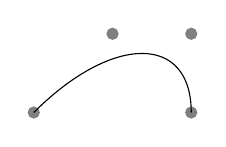
\begin{tikzpicture}
    \filldraw [gray] (0,0) circle [radius=2pt]
            (1,1) circle [radius=2pt]
            (2,1) circle [radius=2pt]
            (2,0) circle [radius=2pt];
    \draw (0,0) .. controls (1,1) and (2,1) .. (2,0);
    \end{tikzpicture}
    \end{lstlisting}%
    \end{minipage}
    \begin{minipage}{0.45\textwidth}
    \centering
    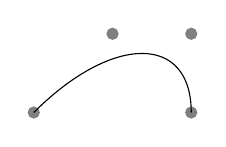
\begin{tikzpicture}
            \filldraw [gray] (0,0) circle [radius=2pt]
                   (1,1) circle [radius=2pt]
                   (2,1) circle [radius=2pt]
                   (2,0) circle [radius=2pt];
            \draw (0,0) .. controls (1,1) and (2,1) .. (2,0);
        \end{tikzpicture}
    \end{minipage}
    \end{figure}

    因此卡尔采用这曲线绘制种方式,仅仅通过精确调整曲线绘制参数实现了半圆的绘制。卡尔对结果颇感满意,但发现以这种方式指定圆形绘制极其繁琐。
    \begin{figure}[!hpbt]
    \begin{minipage}{0.5\textwidth}
    \centering
    \begin{lstlisting}[language=tex]
    \begin{tikzpicture}
        \draw (-1.5,0) -- (1.5,0);
        \draw (0,-1.5) -- (0,1.5);
        \draw (-1,0) .. controls (-1,0.555) and (-0.555,1) .. (0,1)
               .. controls (0.555,1) and (1,0.555) .. (1,0);
    \end{tikzpicture}
    \end{lstlisting}%
    \end{minipage}
    \begin{minipage}{0.45\textwidth}
    \centering
    \begin{tikzpicture}
        \draw (-1.5,0) -- (1.5,0);
        \draw (0,-1.5) -- (0,1.5);
        \draw (-1,0) .. controls (-1,0.555) and (-0.555,1) .. (0,1)
               .. controls (0.555,1) and (1,0.555) .. (1,0);
    \end{tikzpicture}
    \end{minipage}
    \end{figure}

    

    \item \emph{圆路径创建} ~~幸运的是,存在更为简洁的实现方式。我们可使用路径构建操作符\texttt{circle}简洁高效准确地绘制圆形。操作符\texttt{circle}后接方括号以包裹半径值(如下例所示)。需注意:该操作会将当前路径点作为圆心。
    \begin{figure}[!hpbt]
    \begin{minipage}{0.5\textwidth}
    \begin{lstlisting}[language=tex]
    \tikz \draw (0,0) circle [radius=10pt];
    \end{lstlisting}%
    \end{minipage}
    \begin{minipage}{0.45\textwidth}
    \centering
    \tikz \draw (0,0) circle [radius=10pt];
    \end{minipage}
    \end{figure}

    此外,您还可通过ellipse操作符向路径追加椭圆。该操作需指定两个半径值(而非单个半径),语法如下:
    \begin{figure}[!hpbt]
    \begin{minipage}{0.5\textwidth}
    \begin{lstlisting}[language=tex]
    \tikz \draw (0,0) ellipse [x radius=20pt, y radius=10pt];
    \end{lstlisting}%
    \end{minipage}
    \begin{minipage}{0.45\textwidth}
    \centering
    \tikz \draw (0,0) ellipse [x radius=20pt, y radius=10pt];
    \end{minipage}
    \end{figure}

    要绘制轴线非水平或垂直方向的椭圆(即类似右图的"旋转椭圆"),您可运用旋转变换实现(变换机制将在后续章节详解)。这里我们给出绘制代码示例,如下:\begin{verbatim}\tikz \draw[rotate=30] (0,0) ellipse [x radius=6pt, y radius=3pt];\end{verbatim}

    因此,回到卡尔的绘图需求,他只需书写 \texttt{ \backslash draw (0,0) circle [radius=1cm];} 即可完成圆形绘制。然而,卡尔此时警觉地发现:当前圆形尺寸过小,而最终图形需大幅放大。所幸TikZ具备强大的变换选项功能,只需按三倍比例缩放即可轻松实现。但为节省此处版面,我们暂保持当前尺寸不变。
    \begin{figure}[!hpbt]
    \begin{minipage}{0.5\textwidth}
    \begin{lstlisting}[language=tex]
    \begin{tikzpicture}
    \draw (-1.5,0) -- (1.5,0);
    \draw (0,-1.5) -- (0,1.5);
    \draw (0,0) circle [radius=1cm];
    \end{tikzpicture}
    \end{lstlisting}%
    \end{minipage}
    \begin{minipage}{0.45\textwidth}
    \centering
    \begin{tikzpicture}
    \draw (-1.5,0) -- (1.5,0);
    \draw (0,-1.5) -- (0,1.5);
    \draw (0,0) circle [radius=1cm];
    \end{tikzpicture}
    \end{minipage}
    \end{figure}

    
    \item \emph{长方形路径创建} ~~接下来我们需要添加背景网格。存在多种实现方案,例如绘制大量矩形。鉴于矩形应用广泛,TikZ提供了专用语法:向当前路径追加矩形时,请使用\texttt{rectangle}路径构建操作符。该操作符需后接另一坐标点,系统将自动把前一坐标点与当前坐标点作为矩形对角顶点,构建矩形路径。因此,让我们在图形中添加两个矩形示例:
    \begin{figure}[!hpbt]
    \begin{minipage}{0.5\textwidth}
    \begin{lstlisting}[language=tex]
    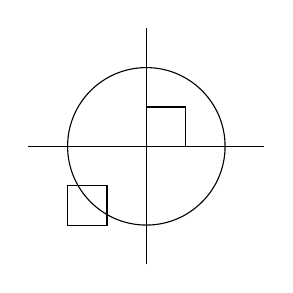
\begin{tikzpicture}
    \draw (-1.5,0) -- (1.5,0);
    \draw (0,-1.5) -- (0,1.5);
    \draw (0,0) circle [radius=1cm];
    \draw (0,0) rectangle (0.5,0.5);
    \draw (-0.5,-0.5) rectangle (-1,-1);
    \end{tikzpicture}
    \end{lstlisting}%
    \end{minipage}
    \begin{minipage}{0.45\textwidth}
    \centering
    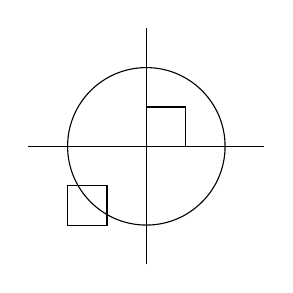
\begin{tikzpicture}
    \draw (-1.5,0) -- (1.5,0);
    \draw (0,-1.5) -- (0,1.5);
    \draw (0,0) circle [radius=1cm];
    \draw (0,0) rectangle (0.5,0.5);
    \draw (-0.5,-0.5) rectangle (-1,-1);
    \end{tikzpicture}
    \end{minipage}
    \end{figure}

    尽管通过矩形命令绘制网格是一个理论可行的方法,但是对于类似卡尔这种绘制较多矩形构成网格的问题不是一个好的解决方案,并且这种方法无法实现"未闭合"的边界。因此卡尔的问题遇到了一点困难。正当卡尔欲采用另一种笨办法——使用 \backslash draw 命令直接绘制四条横竖直线时,却意外发现存在专用的grid路径构建操作符。

    \item \emph{网格形路径创建} ~~grid路径操作符可在当前路径中添加网格。该操作会以前一坐标点为起点,后接坐标点为终点形成一个矩形区域,并自动为该矩形区域生成填充的网格线。例如,代码
    \begin{verbatim}
        \tikz \draw[step=2pt] (0,0) grid (10pt,10pt);
    \end{verbatim} 
    将生成如右图所示的网格(请注意通过 \backslash draw 的可选参数step可定义网格间距,另有xstep与ystep参数可分别设置横纵间距)。卡尔很快会发现,这类参数能实现丰富的样式控制。

    针对卡尔的需求,可采用以下代码实现:
    \begin{figure}[!hpbt]
    \begin{minipage}{0.5\textwidth}
    \begin{lstlisting}[language=tex]
    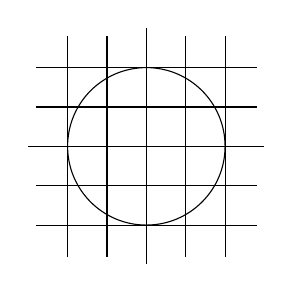
\begin{tikzpicture}
    \draw (-1.5,0) -- (1.5,0);
    \draw (0,-1.5) -- (0,1.5);
    \draw (0,0) circle [radius=1cm];
    \draw[step=.5cm] (-1.4,-1.4) grid (1.4,1.4);
    \end{tikzpicture}
    \end{lstlisting}%
    \end{minipage}
    \begin{minipage}{0.45\textwidth}
    \centering
    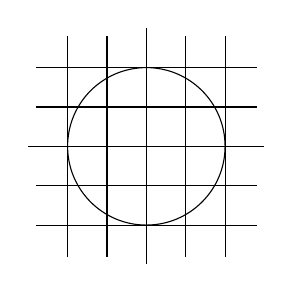
\begin{tikzpicture}
    \draw (-1.5,0) -- (1.5,0);
    \draw (0,-1.5) -- (0,1.5);
    \draw (0,0) circle [radius=1cm];
    \draw[step=.5cm] (-1.4,-1.4) grid (1.4,1.4);
    \end{tikzpicture}
    \end{minipage}
    \end{figure}

    再次审视目标图形时,卡尔意识到网格线应当更加淡化(其子曾提醒:未经淡化的网格线容易分散注意力)。为此,他在绘制网格的\backslash draw命令中追加两个参数:首先将线条颜色设为灰色,其次将线宽调整为极细。最终调整命令顺序,优先绘制网格使其成为底层元素。
    \begin{figure}[!hpbt]
    \begin{minipage}{0.5\textwidth}
    \begin{lstlisting}[language=tex]
    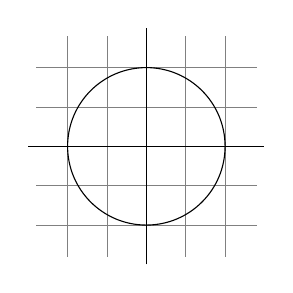
\begin{tikzpicture}
    \draw[step=.5cm,gray,very thin] (-1.4,-1.4) grid (1.4,1.4);
    \draw (-1.5,0) -- (1.5,0);
    \draw (0,-1.5) -- (0,1.5);
    \draw (0,0) circle [radius=1cm];
    \end{tikzpicture}
    \end{lstlisting}%
    \end{minipage}
    \begin{minipage}{0.45\textwidth}
    \centering
    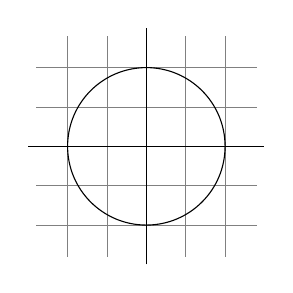
\begin{tikzpicture}
    \draw[step=.5cm,gray,very thin] (-1.4,-1.4) grid (1.4,1.4);
    \draw (-1.5,0) -- (1.5,0);
    \draw (0,-1.5) -- (0,1.5);
    \draw (0,0) circle [radius=1cm];
    \end{tikzpicture}
    \end{minipage}
    \end{figure}

    \item \emph{样式化应用技巧} ~~卡尔可采用预定义样式help lines 替代直接使用gray,very thin参数。样式是预置的绘图参数集合,能系统化管理图形外观。调用help lines即表示"使用预设的辅助线绘制样式"。若卡尔后续想将网格线改为半透明蓝色(blue!50),只需在任意位置添加如下样式定义:
    \begin{verbatim} help lines/.style={color=blue!50,very thin} \end{verbatim}
    该"样式设定器"的效果是:在当前作用域或环境中,help lines选项将完全等同于color=blue!50,very thin的参数组合。

    使用样式能显著提升图形代码的灵活性,让您以统一的方式轻松调整外观效果。通常建议在\{tikzpicture\}环境起始处定义样式,但若需全文档统一风格,可在文档导言区使用 \backslash tikzset命令进行全局样式定义:
    \begin{verbatim} \tikzset{help lines/.style=very thin} \end{verbatim}

    要构建层级化的样式体系,您可以让一个样式继承另一个样式的特性。例如,若卡尔需要基于标准网格样式创建专属的"Karl's grid"样式,可通过以下方式定义
    \begin{verbatim} 
        \tikzset{Karl's grid/.style={help lines,color=blue!50}}
        ...
        \draw[Karl's grid] (0,0) grid (5,5);
    \end{verbatim}

    通过参数化机制,样式的功能变得更加强大。这意味着样式可以像其他选项一样接收参数。例如,卡尔可以将其网格样式参数化——默认显示为蓝色,同时保留切换其他颜色的灵活性:
    \begin{verbatim} 
    \begin{tikzpicture}
    [Karl's grid/.style ={help lines,color=#1!50},
    Karl's grid/.default=blue]

    \draw[Karl's grid]     (0,0) grid (1.5,2);
    \draw[Karl's grid=red] (2,0) grid (3.5,2);
    \end{tikzpicture}
    \end{verbatim}

    在此示例中,`Karl's grid`样式被定义为 \{tikzpicture\}环境的可选参数。如需为其他元素添加样式,只需以逗号分隔继续追加。当存在多个样式定义时,环境的可选参数长度很可能超过实际的绘图内容本身。

    \item \emph{绘图选项} ~~
    卡尔希望了解影响路径绘制的其他选项。他已发现color=⟨颜色⟩可设置线条颜色,而draw=⟨颜色⟩功能类似但更专注——它仅控制线条颜色,填充色可单独设定(这在后续绘制角度弧线填充时将用到)。

    他注意到very thin样式生成极细线条。对此卡尔毫不意外,正如他平静接受以下事实:thin生成细线,thick生成粗线,very thick生成加粗线,ultra thick生成超粗线,而ultra thin生成的线条则细到低分辨率打印设备和显示器难以呈现。此刻他思考:究竟何种选项能产生"标准"粗细的线条?事实证明thin正是正确选择——其粗细与 \TeX 的 \backslash hrule命令完全一致。不过卡尔仍想探究是否存在介于细线与粗线之间的"中间值"。答案是肯定的:semithick。

    另一种实用的线条处理方式是虚线或点线绘制。通过dashed(虚线)与dotted(点线)样式即可实现(效果分别见右图A、B)。这两种样式均提供疏松与致密变体:loosely dashed(疏松虚线)、densely dashed(致密虚线)、loosely dotted(疏松点线)及densely dotted(致密点线)。若确有特殊需求,卡尔还可通过dash pattern选项自定义复杂虚线模式——但其子坚决主张虚线应极度谨慎使用,因过度使用易分散注意力。他断言复杂虚线模式实属糟糕,而卡尔的学生们则对虚线样式毫不在意。

    \vskip \baselineskip
    \item \emph{弧形路径创建} ~~
    当前的技术难点是绘制角度弧线。arc路径构建操作符可解决此需求——它能绘制圆形或椭圆的部分弧段。该操作符后需接方括号包裹的弧线参数,例如arc[start angle=10, end angle=80, radius=10pt]的含义不言自明。卡尔明确需要绘制从 $\alpha$ 到 $\beta$ 的弧线(如右图),其半径应相对较小(约为圆半径的三分之一)。需特别注意:使用arc操作符时,系统将以当前位置为弧线起点进行绘制,因此我们需先定位至起点坐标。
    \begin{figure}[!hpbt]
    \begin{minipage}{0.5\textwidth}
    \begin{lstlisting}[language=tex]
    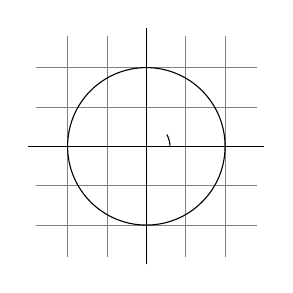
\begin{tikzpicture}
    \draw[step=.5cm,gray,very thin] (-1.4,-1.4) grid (1.4,1.4);
    \draw (-1.5,0) -- (1.5,0);
    \draw (0,-1.5) -- (0,1.5);
    \draw (0,0) circle [radius=1cm];
    \draw (3mm,0mm) arc [start angle=0, end angle=30, radius=3mm];
    \end{tikzpicture}
    \end{lstlisting}%
    \end{minipage}
    \begin{minipage}{0.45\textwidth}
    \centering
    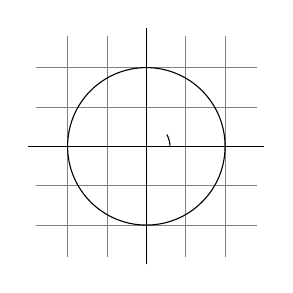
\begin{tikzpicture}
    \draw[step=.5cm,gray,very thin] (-1.4,-1.4) grid (1.4,1.4);
    \draw (-1.5,0) -- (1.5,0);
    \draw (0,-1.5) -- (0,1.5);
    \draw (0,0) circle [radius=1cm];
    \draw (3mm,0mm) arc [start angle=0, end angle=30, radius=3mm];
    \end{tikzpicture}
    \end{minipage}
    \end{figure}

    卡尔认为当前图形确实略显局促,若未掌握缩放技巧将难以继续操作。为此,他可为环境添加[scale=2]缩放选项。虽然可单独应用于每条 \backslash draw命令,但此方案略显繁琐。取而代之的是,将其添加至整个 \{ tikzpicture \} 环境,即可使缩放效果作用于环境内所有元素:
    \begin{figure}[!hpbt]
    \begin{minipage}{0.5\textwidth}
    \begin{lstlisting}[language=tex]
    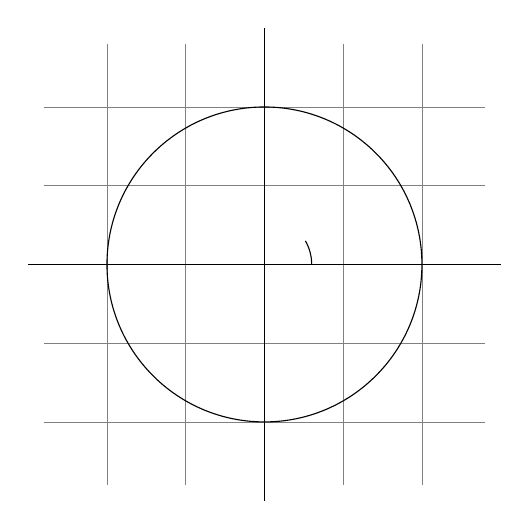
\begin{tikzpicture}[scale=2]
    \draw[step=.5cm,gray,very thin] (-1.4,-1.4) grid (1.4,1.4);
    \draw (-1.5,0) -- (1.5,0);
    \draw (0,-1.5) -- (0,1.5);
    \draw (0,0) circle [radius=1cm];
    \draw (3mm,0mm) arc [start angle=0, end angle=30, radius=3mm];
    \end{tikzpicture}
    \end{lstlisting}%
    \end{minipage}
    \begin{minipage}{0.45\textwidth}
    \centering
    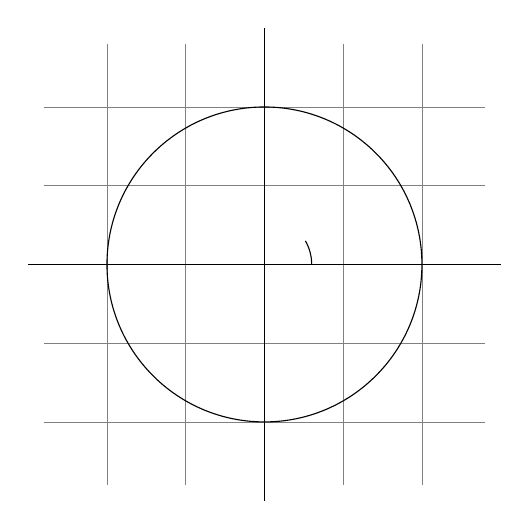
\begin{tikzpicture}[scale=2]
    \draw[step=.5cm,gray,very thin] (-1.4,-1.4) grid (1.4,1.4);
    \draw (-1.5,0) -- (1.5,0);
    \draw (0,-1.5) -- (0,1.5);
    \draw (0,0) circle [radius=1cm];
    \draw (3mm,0mm) arc [start angle=0, end angle=30, radius=3mm];
    \end{tikzpicture}
    \end{minipage}
    \end{figure}

    对于椭圆弧的绘制,您可通过指定"两个"半径参数来实现(区别于标准圆弧的单一半径参数)。例如:
    \begin{figure}[!hpbt]
    \begin{minipage}{0.5\textwidth}
    \begin{lstlisting}[language=tex]
    \tikz \draw (0,0)
    arc [start angle=0, end angle=315,
         x radius=1.75cm, y radius=1cm];
    \end{lstlisting}%
    \end{minipage}
    \begin{minipage}{0.45\textwidth}
    \centering
    \tikz \draw (0,0)
    arc [start angle=0, end angle=315,
         x radius=1.75cm, y radius=1cm];
    \end{minipage}
    \end{figure}
    \item \emph{路径裁剪} ~~
    为精简本手册版面,建议对卡尔的图形进行局部裁剪,从而聚焦呈现"关键"区域。在TikZ中实现裁剪相当便捷:只需使用 \backslash clip命令即可裁剪后续所有绘图内容。该命令语法与 \backslash draw类似,但不会实际绘制路径,而是将给定路径设为裁剪边界作用于后续图形元素。
    \begin{figure}[!hpbt]
    \begin{minipage}{0.5\textwidth}
    \begin{lstlisting}[language=tex]
    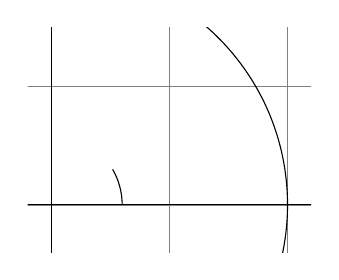
\begin{tikzpicture}[scale=3]
    \clip (-0.1,-0.2) rectangle (1.1,0.75);
    \draw[step=.5cm,gray,very thin] (-1.4,-1.4) grid (1.4,1.4);
    \draw (-1.5,0) -- (1.5,0);
    \draw (0,-1.5) -- (0,1.5);
    \draw (0,0) circle [radius=1cm];
    \draw (3mm,0mm) arc [start angle=0, end angle=30, radius=3mm];
    \end{tikzpicture}
    \end{lstlisting}%
    \end{minipage}
    \begin{minipage}{0.45\textwidth}
    \centering
    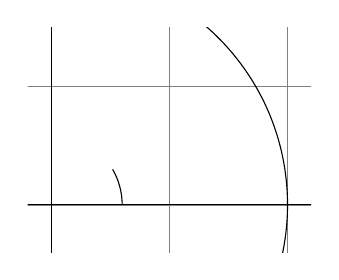
\begin{tikzpicture}[scale=3]
    \clip (-0.1,-0.2) rectangle (1.1,0.75);
    \draw[step=.5cm,gray,very thin] (-1.4,-1.4) grid (1.4,1.4);
    \draw (-1.5,0) -- (1.5,0);
    \draw (0,-1.5) -- (0,1.5);
    \draw (0,0) circle [radius=1cm];
    \draw (3mm,0mm) arc [start angle=0, end angle=30, radius=3mm];
    \end{tikzpicture}
    \end{minipage}
    \end{figure}

    您可同时实现路径绘制与裁剪的双重操作:使用 \backslash draw命令并添加clip选项即可实现(注意:此非完整方案——您也可使用 \backslash clip命令添加draw选项。严格来说,\backslash draw本质是 \backslash path[draw]的简写形式,\backslash clip则是 \backslash path[clip]的简写,因此更底层的实现是 \backslash path[draw,clip])。示例如下:
    \begin{figure}[!hpbt]
    \begin{minipage}{0.5\textwidth}
    \begin{lstlisting}[language=tex]
    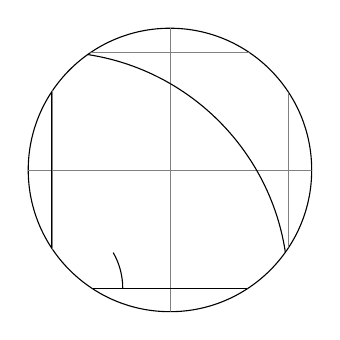
\begin{tikzpicture}[scale=3]
    \clip[draw] (0.5,0.5) circle (.6cm);
    \draw[step=.5cm,gray,very thin] (-1.4,-1.4) grid (1.4,1.4);
    \draw (-1.5,0) -- (1.5,0);
    \draw (0,-1.5) -- (0,1.5);
    \draw (0,0) circle [radius=1cm];
    \draw (3mm,0mm) arc [start angle=0, end angle=30, radius=3mm];
    \end{tikzpicture}
    \end{lstlisting}%
    \end{minipage}
    \begin{minipage}{0.45\textwidth}
    \centering
    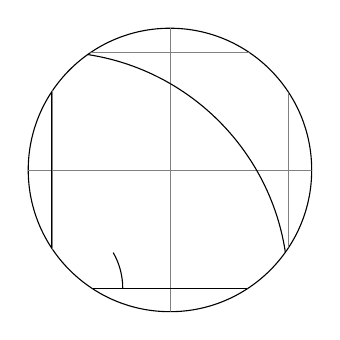
\begin{tikzpicture}[scale=3]
    \clip[draw] (0.5,0.5) circle (.6cm);
    \draw[step=.5cm,gray,very thin] (-1.4,-1.4) grid (1.4,1.4);
    \draw (-1.5,0) -- (1.5,0);
    \draw (0,-1.5) -- (0,1.5);
    \draw (0,0) circle [radius=1cm];
    \draw (3mm,0mm) arc [start angle=0, end angle=30, radius=3mm];
    \end{tikzpicture}
    \end{minipage}
    \end{figure}
    \item \emph{抛物线与正弦路径构建} ~~
    尽管卡尔当前绘图无需这些功能,但他欣喜地发现TikZ提供parabola、sin和cos路径操作符,可在当前路径中追加抛物线及正弦/余弦曲线。抛物线操作的核心特性:当前路径点与操作符后指定的点必在抛物线上。参考以下示例
    \begin{figure}[!hpbt]
    \begin{minipage}{0.5\textwidth}
    \begin{lstlisting}[language=tex]
    \tikz \draw (0,0) rectangle (1,1)  (0,0) parabola (1,1);
    \end{lstlisting}%
    \end{minipage}
    \begin{minipage}{0.45\textwidth}
    \centering
    \tikz \draw (0,0) rectangle (1,1)  (0,0) parabola (1,1);
    \end{minipage}
    \end{figure}

    您还可将弯曲点置于非对称位置:
    \begin{figure}[!hpbt]
    \begin{minipage}{0.5\textwidth}
    \begin{lstlisting}[language=tex]
    \tikz \draw[x=1pt,y=1pt] (0,0) parabola bend (4,16) (6,12);
    \end{lstlisting}%
    \end{minipage}
    \begin{minipage}{0.45\textwidth}
    \centering
    \tikz \draw[x=1pt,y=1pt] (0,0) parabola bend (4,16) (6,12);
    \end{minipage}
    \end{figure}

    sin与cos操作符可在区间内添加正弦/余弦曲线,以前一当前路径点为曲线起点,并以给定终点为曲线终点。示例如下:
    \begin{figure}[!hpbt]
    \begin{minipage}{0.5\textwidth}
    \begin{lstlisting}[language=tex]
    A sine \tikz \draw[x=1ex,y=1ex] (0,0) sin (1.57,1); curve.
    \end{lstlisting}%
    \end{minipage}
    \begin{minipage}{0.45\textwidth}
    \centering
    A sine \tikz \draw[x=1ex,y=1ex] (0,0) sin (1.57,1); curve.
    \end{minipage}
    \end{figure}
    
    \begin{figure}[!hpbt]
    \begin{minipage}{0.5\textwidth}
    \begin{lstlisting}[language=tex]
    \tikz \draw[x=1.57ex,y=1ex] (0,0) sin (1,1) cos (2,0) sin (3,-1) cos (4,0)
                            (0,1) cos (1,0) sin (2,-1) cos (3,0) sin (4,1);
    \end{lstlisting}%
    \end{minipage}
    \begin{minipage}{0.45\textwidth}
    \centering
    \tikz \draw[x=1.57ex,y=1ex] (0,0) sin (1,1) cos (2,0) sin (3,-1) cos (4,0)
                            (0,1) cos (1,0) sin (2,-1) cos (3,0) sin (4,1);
    \end{minipage}
    \end{figure}

    \vskip \baselineskip
    \item \emph{Filling and Drawing} ~~回到图中,卡尔现在希望用极浅的绿色将这个角"填充"起来。为此他没有使用 \backslash draw 命令,而是改用 \backslash fill 命令。卡尔的操作如下:
    \begin{figure}[!hpbt]
    \begin{minipage}{0.5\textwidth}
    \begin{lstlisting}[language=tex]
    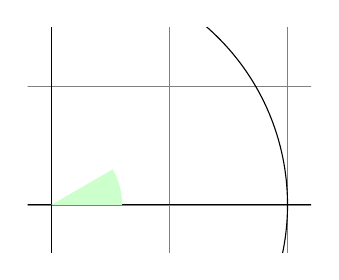
\begin{tikzpicture}[scale=3]
    \clip (-0.1,-0.2) rectangle (1.1,0.75);
    \draw[step=.5cm,gray,very thin] (-1.4,-1.4) grid (1.4,1.4);
    \draw (-1.5,0) -- (1.5,0);
    \draw (0,-1.5) -- (0,1.5);
    \draw (0,0) circle [radius=1cm];
    \fill[green!20!white] (0,0) -- (3mm,0mm)
        arc [start angle=0, end angle=30, radius=3mm] -- (0,0);
    \end{tikzpicture}
    \end{lstlisting}%
    \end{minipage}
    \begin{minipage}{0.45\textwidth}
    \centering
    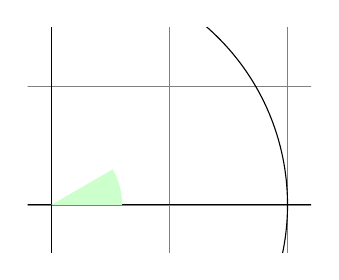
\begin{tikzpicture}[scale=3]
    \clip (-0.1,-0.2) rectangle (1.1,0.75);
    \draw[step=.5cm,gray,very thin] (-1.4,-1.4) grid (1.4,1.4);
    \draw (-1.5,0) -- (1.5,0);
    \draw (0,-1.5) -- (0,1.5);
    \draw (0,0) circle [radius=1cm];
    \fill[green!20!white] (0,0) -- (3mm,0mm)
        arc [start angle=0, end angle=30, radius=3mm] -- (0,0);
    \end{tikzpicture}
    \end{minipage}
    \end{figure}

    颜色表达式 green!20!white 表示 20\% 绿色与 80\% 白色混合(即 20\% 绿色 + 80\% 白色)。之所以能使用此类色彩表达式,是因为 TikZ 底层采用了 Uwe Kern 开发的 xcolor 宏包,具体色彩表达式说明可参阅该宏包的文档。

    如果卡尔最后没有用 \texttt{--(0,0)} 来"闭合"路径会怎样?实际上路径会自动闭合,因此这步操作可以省略。事实上,采用以下写法甚至更为理想
    \begin{verbatim} 
    \fill[green!20!white] (0,0) -- (3mm,0mm)
        arc [start angle=0, end angle=30, radius=3mm] -- cycle;
    \end{verbatim}

    \texttt{--cycle} 指令会将当前路径(实际上是当前路径的当前分段)的首尾点平滑连接形成闭合路径。为直观理解其差异,请看以下示例:
    \begin{figure}[!hpbt]
    \begin{minipage}{0.5\textwidth}
    \begin{lstlisting}[language=tex]
    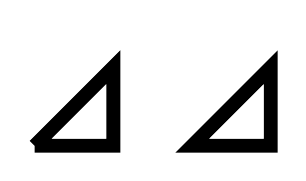
\begin{tikzpicture}[line width=5pt]
        \draw (0,0) -- (1,0) -- (1,1) -- (0,0);
        \draw (2,0) -- (3,0) -- (3,1) -- cycle;
        \useasboundingbox (0,1.5); % make bounding box higher
    \end{tikzpicture}
    \end{lstlisting}%
    \end{minipage}
    \begin{minipage}{0.45\textwidth}
    \centering
    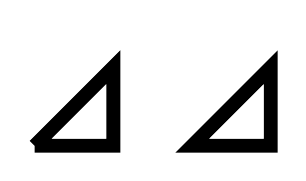
\begin{tikzpicture}[line width=5pt]
        \draw (0,0) -- (1,0) -- (1,1) -- (0,0);
        \draw (2,0) -- (3,0) -- (3,1) -- cycle;
        \useasboundingbox (0,1.5); % make bounding box higher
    \end{tikzpicture}
    \end{minipage}
    \end{figure}

    还可以使用 \backslash filldraw 命令同时执行填充和绘制路径的双重操作。该命令会先绘制路径轮廓,再进行内部填充。初看似乎作用有限,但关键在于可为填充色(fill)和描边色(stroke)分别指定不同颜色。具体通过如下可选参数实现:
    \begin{figure}[!hpbt]
    \begin{minipage}{0.5\textwidth}
    \begin{lstlisting}[language=tex]
    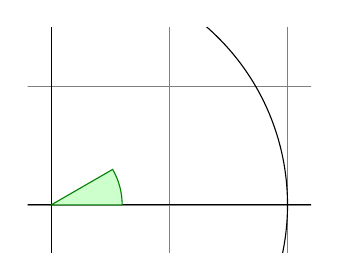
\begin{tikzpicture}[scale=3]
        \clip (-0.1,-0.2) rectangle (1.1,0.75);
        \draw[step=.5cm,gray,very thin] (-1.4,-1.4) grid (1.4,1.4);
        \draw (-1.5,0) -- (1.5,0);
        \draw (0,-1.5) -- (0,1.5);
        \draw (0,0) circle [radius=1cm];
        \filldraw[fill=green!20!white, draw=green!50!black] (0,0) -- (3mm,0mm)
            arc [start angle=0, end angle=30, radius=3mm] -- cycle;
    \end{tikzpicture}
    \end{lstlisting}%
    \end{minipage}
    \begin{minipage}{0.45\textwidth}
    \centering
    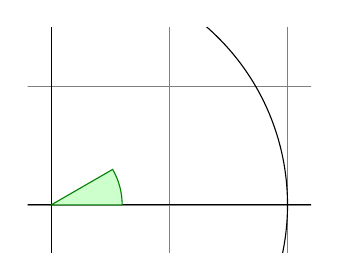
\begin{tikzpicture}[scale=3]
        \clip (-0.1,-0.2) rectangle (1.1,0.75);
        \draw[step=.5cm,gray,very thin] (-1.4,-1.4) grid (1.4,1.4);
        \draw (-1.5,0) -- (1.5,0);
        \draw (0,-1.5) -- (0,1.5);
        \draw (0,0) circle [radius=1cm];
        \filldraw[fill=green!20!white, draw=green!50!black] (0,0) -- (3mm,0mm)
            arc [start angle=0, end angle=30, radius=3mm] -- cycle;
    \end{tikzpicture}
    \end{minipage}
    \end{figure}

    \item \emph{阴影} ~~卡尔短暂考虑过通过着色让这个角显得"更花哨"。与使用单一纯色填充区域不同,着色可实现不同颜色间的平滑渐变。命令如下:
    \begin{figure}[!hpbt]
    \begin{minipage}{0.5\textwidth}
    \begin{lstlisting}[language=tex]
       \tikz \shade (0,0) rectangle (2,1)  (3,0.5) circle (.5cm);
    \end{lstlisting}%
    \end{minipage}
    \begin{minipage}{0.45\textwidth}
    \centering
       \tikz \shade (0,0) rectangle (2,1)  (3,0.5) circle (.5cm);
    \end{minipage}
    \end{figure}
     
    默认着色效果是从灰色到白色的平滑渐变。若需指定其他颜色,可通过以下选项参数实现:
    \begin{figure}[!hpbt]
    \begin{minipage}{0.5\textwidth}
    \begin{lstlisting}[language=tex]
    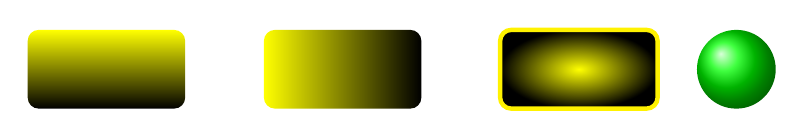
\begin{tikzpicture}[rounded corners,ultra thick]
        \shade[top color=yellow,bottom color=black] (0,0) rectangle +(2,1);
        \shade[left color=yellow,right color=black] (3,0) rectangle +(2,1);
        \shadedraw[inner color=yellow,outer color=black,draw=yellow] (6,0) rectangle +(2,1);
        \shade[ball color=green] (9,.5) circle (.5cm);
    \end{tikzpicture}
    \end{lstlisting}%
    \end{minipage}
    \begin{minipage}{0.45\textwidth}
    \centering
    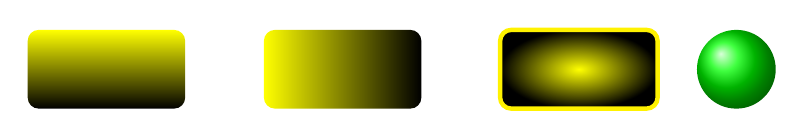
\begin{tikzpicture}[rounded corners,ultra thick]
        \shade[top color=yellow,bottom color=black] (0,0) rectangle +(2,1);
        \shade[left color=yellow,right color=black] (3,0) rectangle +(2,1);
        \shadedraw[inner color=yellow,outer color=black,draw=yellow] (6,0) rectangle +(2,1);
        \shade[ball color=green] (9,.5) circle (.5cm);
    \end{tikzpicture}
    \end{minipage}
    \end{figure}

    对于卡尔的任务,下面的做法更合适。
    \begin{figure}[!hpbt]
    \begin{minipage}{0.5\textwidth}
    \begin{lstlisting}[language=tex]
    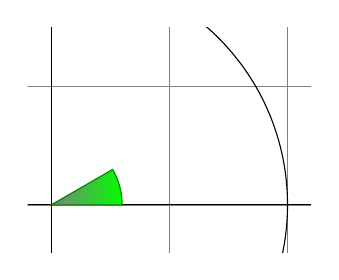
\begin{tikzpicture}[scale=3]
        \clip (-0.1,-0.2) rectangle (1.1,0.75);
        \draw[step=.5cm,gray,very thin] (-1.4,-1.4) grid (1.4,1.4);
        \draw (-1.5,0) -- (1.5,0);
        \draw (0,-1.5) -- (0,1.5);
        \draw (0,0) circle [radius=1cm];
        \shadedraw[left color=gray,right color=green, draw=green!50!black]
            (0,0) -- (3mm,0mm)
            arc [start angle=0, end angle=30, radius=3mm] -- cycle;
    \end{tikzpicture}
    \end{lstlisting}%
    \end{minipage}
    \begin{minipage}{0.45\textwidth}
    \centering
    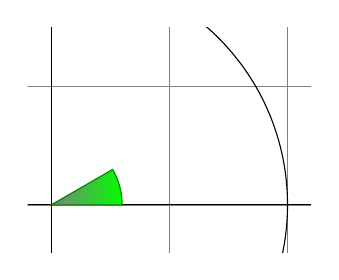
\begin{tikzpicture}[scale=3]
        \clip (-0.1,-0.2) rectangle (1.1,0.75);
        \draw[step=.5cm,gray,very thin] (-1.4,-1.4) grid (1.4,1.4);
        \draw (-1.5,0) -- (1.5,0);
        \draw (0,-1.5) -- (0,1.5);
        \draw (0,0) circle [radius=1cm];
        \shadedraw[left color=gray,right color=green, draw=green!50!black]
            (0,0) -- (3mm,0mm)
            arc [start angle=0, end angle=30, radius=3mm] -- cycle;
    \end{tikzpicture}
    \end{minipage}
    \end{figure}
    然而他明智地决定放弃着色——通常这类效果徒增干扰,对图形表达反而无益。
    \item \emph{指定坐标} ~~卡尔接下来要添加正弦和余弦线。他已知晓可用 color= 选项设置线条颜色,那么如何最优指定坐标位置呢?

    坐标指定存在多种方式。最简易的方法是直接使用 $(10pt,2cm)$ 这类表达式,表示 x轴方向$10pt$、$y$轴方向$2cm$。另一种方式是省略单位写成 $(1,2)$,其含义为"当前$x$向量的$1$倍与当前$y$向量的$2$倍之和"。这两个向量默认值分别为:$x$轴方向$1cm$,$y$轴方向$1cm$。

    要指定极坐标点,可使用 (30:1cm) 格式,表示30度方向上1cm处的点——这在定位"圆周上的点"时尤为实用。

    若在坐标前添加单个"$+$"或双"$++$"符号,如 $+(0cm,1cm)$ 或 $++(2cm,0cm)$,其语义有本质差异:(1)$+$前缀表示“相对前一个坐标点上移$1cm$”;(2) $++$ 前缀表示“相对前一个坐标点右移$2cm$,并将该点更新为新的当前点”。
    \begin{figure}[!hpbt]
    \begin{minipage}{0.5\textwidth}
    \begin{lstlisting}[language=tex]
    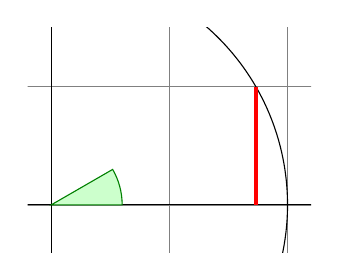
\begin{tikzpicture}[scale=3]
        \clip (-0.1,-0.2) rectangle (1.1,0.75);
        \draw[step=.5cm,gray,very thin] (-1.4,-1.4) grid (1.4,1.4);
        \draw (-1.5,0) -- (1.5,0);
        \draw (0,-1.5) -- (0,1.5);
        \draw (0,0) circle [radius=1cm];
        \filldraw[fill=green!20,draw=green!50!black] (0,0) -- (3mm,0mm)
            arc [start angle=0, end angle=30, radius=3mm] -- cycle;
        \draw[red,very thick] (30:1cm) -- +(0,-0.5);
    \end{tikzpicture}
    \end{lstlisting}%
    \end{minipage}
    \begin{minipage}{0.45\textwidth}
    \centering
    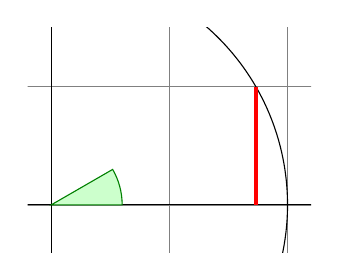
\begin{tikzpicture}[scale=3]
        \clip (-0.1,-0.2) rectangle (1.1,0.75);
        \draw[step=.5cm,gray,very thin] (-1.4,-1.4) grid (1.4,1.4);
        \draw (-1.5,0) -- (1.5,0);
        \draw (0,-1.5) -- (0,1.5);
        \draw (0,0) circle [radius=1cm];
        \filldraw[fill=green!20,draw=green!50!black] (0,0) -- (3mm,0mm)
            arc [start angle=0, end angle=30, radius=3mm] -- cycle;
        \draw[red,very thick] (30:1cm) -- +(0,-0.5);
    \end{tikzpicture}
    \end{minipage}
    \end{figure}

\end{enumerate}





%\section{机器学习绘图}



\chapter{表格}\label{cha:table}
引入样式宏包cnbasesetup.sty时,传入\verb|tab|参数引入表格绘制的宏包。
\begin{verbatim}
    \usepackage[super,tikz,tab,list,math]{style/cnbasesetup}
\end{verbatim}

\section{表格的定义环境}\label{sec:table-def-env}


\verb|tabular|及\verb|tabular*|环境是表格绘制的基本环境。tabular 环境可以用来排版带有横线和竖线的表格,\LaTeX 自动确定表格的宽度。tabular*环境与 tabular 环境类似,只是可以用参数指定表格的整体宽度,此外列参数必须在第一列后面的某个地方包含一个合适的表达式 (见下面说明)\footnote{在数学模式下使用的 array 环境的语法和参数的意义与 tabular 环境中的完全一样}。他们的语法格式如下:
\begin{verbatim}
    \begin{tabular}[位置可选参数]{列格式参数}
    每行由\\划分
    \end{tabular}
    \begin{tabular*}{宽度}[位置可选参数]{列格式参数}
    每行由\\划分
\end{tabular*}
\end{verbatim}



\section{表格环境参数格式}
\parwords{位置可选参数}
当然,有些时候我们需要更细致地控制表格的位置。\verb|table|环境中额外的位置控制参数为我们提供了一套控制表格位置的方法。下面我们给出一个简单的例子。
\begin{table}[!hpbt]
    \caption[表格插入位置控制选项]{\enspace 表格插入位置控制选项}
    \label{tab:table-position-options}
    \centering
    \normalsize% fontsize 
    \setlength{\tabcolsep}{4pt}% column separation
    \begin{tabular}{ll}
    \toprule
    选项 & 位置 \\
    \midrule
    h	& 将浮动元素的位置设定为 here\\
    t	& 将浮动元素的位置设定为页面的上方(top)\\
    b	& 将浮动元素的位置设定为页面的底部(bottom)\\
    p	& 将浮动元素仅放置在一个特殊的页面\\
    !	& 重新设置 \LaTeX{} 的一个内部参数\\
    H	& 浮动元素精确地放置在文本中所出现的位置\\
    \bottomrule
    \end{tabular}
\end{table}
其中, \verb|\begin{table}[h]|,方括号中的参数 \verb|h| 意味着 here,即大约插入到当前上下文位置,而不是完全精确地插入到给定位置。 参数 \verb|!| 决定了 \LaTeX{} 如何判断一个浮动元素的位置够不够“好”,参数 H 需要引入float包,它有可能会造成一些错误,有时候等价于h!。表~\ref{tab:table-position-options}~中列出了参数的可选值。总之,\verb|table|环境位置控制参数与 \verb|figure| 环境一致。

\parwords{列必选参数}
这个参数控制表格的列格式,故又称为列格式参数。在这个参数中,对每一列必须有一个相应的格式符号,另外还可能包含相应于表格左右边界和列间距的其它项。列格式符号可以取下列值:
\begin{table}[!hpbt]
    \caption[表格列格式参数]{\enspace 表格列格式参数}
    \label{tab:table-col-options}
    \centering
    \normalsize% fontsize 
    \setlength{\tabcolsep}{4pt}% column separation
    \begin{tabular}{ll}
    \toprule
    位置参数 & 位置 \\
    \midrule
    l	& 列中文本左对齐\\
    r	& 列中文本右对齐\\
    c	& 列中文本居中\\
    p	& \makecell[l]{宽度: 指定列的文本宽度,由宽度参数给出,\\ 列中文本按该宽度自动换行}\\
    |	& 画一条竖直线\\
    ||	& 画二条紧相邻的竖直线\\
    *\{num\}\{col-format\}& \makecell[l]{包含在col-format中的列格式被复制成num份,\\ 例如 *\{5\}\{|c\} 等价于 \texttt{|c|c|c|c|c}}\\
    \bottomrule
    \end{tabular}
\end{table}

\section{表格文本行中的命令}
表格中的每一水平行都由 \verb|\\| 结束。这些行由一组彼此之间用 \& 符号分开的列条目组
成。因此每一行应具有与列定义中列中相同数目的列条目,其中有些条目可以是空白的。
\begin{enumerate}
    \item \emph{ \backslash tabularnewline 命令}~~ \verb|\tabularnewline| 命令用于强制表格中一行的结束,而 \backslash\backslash 除了可以结束整个一行表格内容外,还可以在单个列的内容中实现换行。
    \item \emph{ \backslash hline 命令}~~ 这条命令只能位于第一行前面或紧接在行结束命令 \verb|\\| 的后面,表示在刚结束的那一行画一根水平的直线。如果这条命令位于表格的开头,那么就会在表格顶部画一横线,横线的宽度与表格的宽度相同。 放在一起的两条水平 \verb|\hline| 命令就会画出两条间隔很小的水平线。
    \item \emph{ \backslash cline\{n-m\}  命令}~~ \verb|\cline{n-m}| 命令的放置同 \verb|\hline| 命令,并且在一行中可以出现多次。该命令从第 n 列的左边开始,画一条到第 m 列右边结束的水平线。
    \item \emph{ \backslash vline 命令}~~ 该命令画一条竖直线,其高度等于其所在行的行高。用这种命令,可以得到那些不是贯穿整个表格的竖直线。
    \item \emph{ \backslash multicolumn\{列数\}\{ALIGNMENT\}\{CONTENT\} 命令}~~ 该命令用于合并列单元格,并可以在合并的单元格内进行内容的对齐,即该表格单元占据的列数,ALIGNMENT代表表格内容的对齐方式(填*,l,c或者r),CONTENT则是表格单元里的内容。例如,\backslash multicolumn\{3\}\{|c|\}\{内容\} 表示将内容合并到三列,并居中对齐。
    \item \emph{ \backslash multirow 命令}~~ 该命令用于合并行单元格,并可以在合并的单元格内进行内容的对齐,其基本语法为:
    \begin{verbatim} \multirow[⟨vpos⟩]{⟨nrows⟩}[⟨bigstruts⟩]{⟨width⟩}[⟨vmove⟩]{⟨text⟩} \end{verbatim}
    
    其中参数意义如下:
    \begin{itemize}
        \item \verb|⟨vpos⟩|~ 定义了合并后单元格内文本竖直位置的对齐方式,参数 \verb|t| 表示顶部对齐, \verb|b| 表底部部对齐,\verb|c|表示居中对齐,缺省默认值为 \verb|b|;
        \item \verb|⟨nrows⟩|~ 定义了合并后单元格纵向跨越的行数。该列的其他行必须留空,否则 \verb|\multirow| 创建的内容会覆盖已有数据。当 \verb|⟨nrows⟩| 为正值时,纵向范围涵盖当前行及下方 \verb|(⟨nrows⟩-1)| 行;为负值时则涵盖当前行及上方 \verb|(-⟨nrows⟩-1)| 行;\verb|⟨nrows⟩| 允许使用分数值,便于进行精细调整;
        \item \verb|⟨bigstruts⟩|~  参数主要在使用 bigstrut 宏包时生效。其数值表示跨行区域内所有 \verb|\bigstrut| 命令的使用次数总和。具体计数规则为:(1)无参数版本 \verb|\bigstrut| 计为 2 次,(2)带位置参数的 \verb|\bigstrut[⟨x⟩]|(\verb|⟨x⟩|为 \verb|t| 或 \verb|b|)计为 1 次,默认值为 0;\verb|⟨bigstruts⟩| 参数可添加字母前缀(\verb|t|、\verb|b| 或 \verb|tb|)实现精细控制(详细内容参见 \href{https://texdoc.org/serve/multirow.pdf/0}{multirow宏包文档});字母与数值间可保留空格,格式为 \verb|t 3| 或 \verb|tb 2|;
        \item \verb|⟨width⟩|~ 参数指定文本排版宽度,特殊取值包括:(1) \verb|*| 表示采用文本的自然宽度,(2) \verb|=| 表示采用当前列(即 \verb|\multirow| 条目所在列)的预设宽度;
        \item \verb|⟨vmove⟩|~ 是用于微调的长度值:文本将在原始位置基础上,根据该长度值上移(若 \verb|⟨vmove⟩| 为负值则下移);
        \item \verb|⟨text⟩|~ 为实际文本内容。根据宽度设定方式不同,排版规则如下:(1)如果显式指定宽度时,文本将置于指定宽度的 \verb|\parbox| 中,可通过 \\ 强制换行;(2)如果宽度设为 \verb|*| 时,文本以行内模式 (LR mode) 排版,需多行显示时,应在 ⟨text⟩ 内嵌套 tabular 或 array 环境;(3)如果宽度设为 \verb|=| 时,仅当 \verb|\multirow| 条目位于预定义宽度的列中生效(如:\verb|p{}| 列、tabularx 的 X 列、tabulary 的 \verb|L/C/R/J| 列),文本将置于该列预设宽度的 \verb|\parbox| 中,非适用场景使用 \verb|=| 将导致异常(通常表现为列宽过大)。
    \end{itemize}
    \item \emph{ at表达式命令}~~ \verb|@{}|表达式为每行的某两个相邻的列之间插入文本,同时自动去掉原来在这两列之间插入的空白。
    \begin{figure}[!hpbt]
        \begin{minipage}{0.5\textwidth}
        \begin{lstlisting}[language=tex]
        \begin{tabular}{r@{.}l}
        3   & 14159 \\
        16  & 2     \\
        123 & 456   \\
        \end{tabular}
        \end{lstlisting}%
        \end{minipage}
        \begin{minipage}{0.45\textwidth}
        \centering
        \begin{tabular}{r@{.}l}
        3   & 14159 \\
        16  & 2     \\
        123 & 456   \\
        \end{tabular}
        \end{minipage}
    \end{figure}

    对于\verb|@{}|,有下面几点需要说明:
    \begin{itemize}
        \item 如果我们需要继续使用空白,必须在 \verb|@{}| 表达式的文本参数中必须包含 \verb|\hspace{<wsep>}| 命令,或者使用 \verb|!{}| 替换;\verb|<wsep>| 为空白长度,可以是指定的长度(例如 \verb|4pt| )或者弹性长度 \verb|\fill|;
        \begin{figure}[!hpbt]
        \begin{minipage}{0.5\textwidth}
        \begin{lstlisting}[language=tex]
        \begin{tabular}{r@{.\hspace{\fill}}l}
        3   & 14159 \\
        16  & 2     \\
        123 & 456   \\
        \end{tabular}
        \end{lstlisting}%
        \end{minipage}
        \begin{minipage}{0.45\textwidth}
        \centering
        \begin{tabular}{r@{.\hspace{\fill}}l}
        3   & 14159 \\
        16  & 2     \\
        123 & 456   \\
        \end{tabular}
        \end{minipage}
        \end{figure}
        \item 如果希望某两个特定列之间的间隔与缺省的标准间隔不同,可以在表格环境的行参数中相应的位置上放上 \verb|@{\hsapce{<wsep>}}| 控制,此时该处列间间隔将变成 \verb|<wsep>|;
        \begin{figure}[!hpbt]
        \begin{minipage}{0.5\textwidth}
        \begin{lstlisting}[language=tex]
        \begin{tabular}{r@{.\hspace{\fill}}l}
        3   & 14159 \\
        16  & 2     \\
        123 & 456   \\
        \end{tabular}
        \end{lstlisting}%
        \end{minipage}
        \begin{minipage}{0.45\textwidth}
        \centering
        \begin{tabular}{rl}
        3   & 14159 \\
        16  @{.\hspace{\fill}}& 2     \\
        123 & 456   \\
        \end{tabular}
        \end{minipage}
        \end{figure}
        \item \verb|@{}| 表达式中可以使用 \verb|\extracolsep{<wsep>}| 控制,使后面所有列间间隔在原来标准间隔的基础上增加\verb|<wsep>|大小;
        \item 在 \verb|tabular*| 环境中。必须使用 \verb|@{\extracolsep\fill}| 命令,使得后面所有列间距可以伸展到预定义的表格宽度;
        \item 一个表格即使左右边界没有竖线或其他表征符号,相应的位置与后面 (前面) 的列之间也会插入等于标准列间隔一半的空白;如果不希望有这些空白,可以在行参数开始或结束处使用 \verb|@{}| 表达式。
    \end{itemize}
\end{enumerate}


\section{表格浮动体环境}
\texttt{table}环境用于将表格进行浮动处理,使其可以自动调整到合适的位置,并能够添加表格标题和标签。一个简单的表格环境格式如下:
\begin{verbatim}
\begin{table}[位置可选参数]
  \caption{T.}
  \label{table:1}%
    ... ...
\end{table}
\end{verbatim}
这里需要注意:
(1)常用的位置选项与 \verb|figure| 环境一致,如表 \ref{tab:table-position-options} ,包含: \verb|h| :在当前位置放置表格; \verb|t| :将表格放置在页面的顶部; \verb|b| :将表格放置在页面的底部;\verb|p|:单独放置表格到一页等。
(2)给定表标题 \verb|\caption{<短标题>}{<长标题>}| ,可放置在表上方或者下方。
(3)给表打标签 \verb|\label{<标签名称>}| ,表格标签名称一般使用“table:”作为前缀,以方便辨认和分类管理。注意:这个命令必须位于 \verb|\caption|之后。
(4)可以使用命令  \verb|\ref{<标签名称>}| 引用表格,也可以使用命令 \verb|\pageref{<标签名称>}| 定位其所在页码。


\texttt{table}环境用通常与\texttt{tabular}或\texttt{tabular*}搭配使用,\texttt{table}环境控制表格的位置、标题及标签,\texttt{tabular}或\texttt{tabular*}绘制表格。同时,为了使表格在页面上居中,还会利用 center 环境或 \backslash centering 命令:
\begin{verbatim}
\begin{table}[位置可选参数]
  \begin{center}%让表格居中
  \caption{T.}%resnet50 on imagenet1k
  \label{table:1}%
    \begin{tabular}{列格式参数}
    每行由\\划分
    \end{tabular}
  \end{center}
\end{table}
\begin{table}[位置选项]
  \begin{center}%让表格居中
  \caption{T.}%resnet50 on imagenet1k
  \label{table:1}%
    \begin{tabular*}{宽度}{列格式参数}
    每行由\\划分
    \end{tabular*}
  \end{center}
\end{table}
\end{verbatim}


\section{表格样例}
我们先看一个表格样例:
\begin{lstlisting}[language=tex]
    \begin{table}[!htbp]
        \bicaption{这是一个样表。}{This is a sample table.}
        \label{tab:sample}
        \centering
        \footnotesize% fontsize
        \setlength{\tabcolsep}{4pt}% column separation
        \renewcommand{\arraystretch}{1.2}%row space 
        \begin{tabular}{l|cccc>{\columncolor{blue}}cccc}
            \hline
            \rowcolor{gray} 行号 & \multicolumn{8}{c}{跨多列的标题}\\
            \hline
            \cellcolor{red} R1 & $1$ & $2$ & $3$ & $4$ & $5$ & $6$ & $7$ & $8$\\
            R2 & $1$ & $2$ & $3$ & $4$ & $5$ & $6$ & $7$ & $8$\\
            \cline{2-9}% partial hline from column i to column j
            \multirow{2}{l}{R3-4}& $1$ & $2$ & $3$ & $4$ & $5$ & $6$ & $7$ & $8$\\
             & $1$ & $2$ & $3$ & $4$ & $5$ & $6$ & $7$ & \textcolor{red}{$8$}\\
            \hline
        \end{tabular}
    \end{table}
\end{lstlisting}
其中
\begin{itemize}
    \item \texttt{[!htbp]}:表示表格的浮动位置,\texttt{!}表示必须出现在文档的当前位置,\texttt{h}表示在当前位置,\texttt{t}表示在文本顶部,\texttt{b}表示在文本底部,\texttt{p}表示在浮动页。
    \item \texttt{\textbackslash bicaption\{中文标题\}\{英文标题\}}命令用于设置表格的标题,第一个参数为中文标题,第二个参数为英文标题。这个命令的完整版格式为\texttt{\textbackslash bicaption \textbackslash [中文表目录显示标题 \textbackslash ]\{中文标题\}\textbackslash [英文表目录显示标题 \textbackslash ]\{英文标题\}}。
    \item \texttt{\textbackslash label\{标签名\}}命令用于设置表格的标签,标签名可以自定义。
    \item \texttt{\textbackslash centering}命令用于设置表格居中。
    \item \texttt{\textbackslash footnotesize}命令用于设置表格字体大小。
    \item \texttt{\textbackslash tabcolsep\{4pt\}}命令用于设置表格列间距。
    \item \texttt{\textbackslash renewcommand\{\textbackslash arraystretch\}\{1.2\}}命令用于设置表格行间距。
    \item \texttt{\textbackslash begin\{tabular\}\{l|cccc>\{\textbackslash columncolor\{blue\}\}cccc\}}命令用于设置表格单元格中内容对齐方式,\texttt{l}表示左对齐,\texttt{c}表示居中对齐,\texttt{r}表示右对齐, |表示列之间画竖线隔开。\texttt{>\{\textbackslash columncolor\{blue\}\}}表示列的颜色。
    \item \texttt{\textbackslash hline}命令用于设置表格的横线。
    \item \texttt{\textbackslash multicolumn\{8\}\{c\}\{跨多列的标题\}}命令用于设置表格的跨列单元格。
    \item \texttt{\textbackslash multirow\{2\}\{*\}\{Row3-4\}}命令用于设置表格的跨行单元格。
    \item \texttt{\textbackslash cline\{2-9\}}命令用于设置表格的部分横线。
    \item \texttt{\textbackslash \textbackslash}命令用于设置表格的换行。
    \item \texttt{\&}命令用于行内单元格分割。
    \item \texttt{\textbackslash rowcolor\{gray\}}命令用于设置表格的行颜色。
    \item \texttt{\textbackslash cellcolor\{gray\}}命令用于设置表格的单元格颜色。
    \item \texttt{\textbackslash textcolor\{red\}\{红色文字\}}命令用于设置表格的文字颜色。
\end{itemize}
请见表~\ref{tab:sample}(注意:使用命令\texttt{\textbackslash ref\{tab:sample\}}引用表格)。
\begin{table}[!htbp]
    \bicaption{这是一个样表。}{This is a sample table.}
    \label{tab:sample}
    \centering
    \footnotesize% fontsize
    \setlength{\tabcolsep}{4pt}% column separation
    \renewcommand{\arraystretch}{1.2}%row space 
    \begin{tabular}{l|cccc>{\columncolor{blue}}cccc}
        \hline
        \rowcolor{gray} 行号 & \multicolumn{8}{c}{跨多列的标题}\\
        \hline
        \cellcolor{red} R1 & $1$ & $2$ & $3$ & $4$ & $5$ & $6$ & $7$ & $8$\\
        R2 & $1$ & $2$ & $3$ & $4$ & $5$ & $6$ & $7$ & $8$\\
        \cline{2-9}% partial hline from column i to column j
        \multirow[c]{2}*{R3-4}& $1$ & $2$ & $3$ & $4$ & $5$ & $6$ & $7$ & $8$\\
        & $1$ & $2$ & $3$ & $4$ & $5$ & $6$ & $7$ & \textcolor{red}{$8$}\\
        \hline
    \end{tabular}
\end{table}

许多专业排版的书籍和期刊都使用简单的表格,它们在行上下有适当的间距,而且几乎从不使用垂直线。许多 \LaTeX{} 表格示例(包括这本)展示了垂直线的使用(使用“|”)和双线的使用(使用“||”),这些在专业出版物中被认为是不必要的,而且会分散注意力。 booktabs 包可以方便地为  \LaTeX{} 表格提供这种专业性,它的文档 也提供了关于构成“良好”表格的指南。

简而言之,该包使用 \verb|\toprule| 表示最上面的规则(或线), \verb|\midrule| 表示出现在表格中间的规则(例如标题下面的规则), \verb|\bottomrule| 表示最下面的规则。这确保了规则的宽度和间距是可以接受的。此外, \verb|\cmidrule| 可以用来表示跨越指定列的中间规则。

%以下示例对比了 booktabs 的使用和两种等效的正常 LaTeX 实现(第二个示例需要在序言中使用 \verb|\usepackage{array}| 或 \verb|\usepackage{dcolumn}|,第三个示例需要在序言中使用 \verb|\usepackage{booktabs}|)。

\begin{example}三线表是科技期刊与论文常用的表格,本例给出了一种简单的三线表格绘制样例。
\begin{lstlisting}[language=tex]
\begin{table}[!hbtp]
    \caption[峰谷电价]{\enspace 峰谷电价}
    \label{tab:elec-price}
    \centering
    \normalsize% fontsize 
    \setlength{\tabcolsep}{4pt}% column separation
    \begin{tabular}{m{40pt}<{\raggedright}m{120pt}<{\raggedright}m{80pt}<{\raggedright}}
    \toprule
    周期 & 时段 & 电价 (CNY/kWh) \\
    \midrule
    Peak & 12:00--15:00, 18:00--21:00 & 1.3782\\
    Flat & 9:00--10:00, 15:00--18:00, 21:00--23:00 & 0.8595\\
    Valley & 1:00--7:00, 23:00--0:00 & 0.3658\\
    \bottomrule
    \end{tabular}
\end{table}
\end{lstlisting}
其显示效果如表\ref{tab:elec-price}。
\end{example}
\begin{table}[!hbtp]
    \caption[峰谷电价]{\enspace 峰谷电价}
    \label{tab:elec-price}
    \centering
    \normalsize% fontsize 
    \setlength{\tabcolsep}{4pt}% column separation
    \begin{tabular}{m{40pt}<{\raggedright}m{120pt}<{\raggedright}m{80pt}<{\raggedright}}
    \toprule
    周期 & 时段 & 电价 (CNY/kWh) \\
    \midrule
    Peak & 12:00--15:00, 18:00--21:00 & 1.3782\\
    Flat & 9:00--10:00, 15:00--18:00, 21:00--23:00 & 0.8595\\
    Valley & 1:00--7:00, 23:00--0:00 & 0.3658\\
    \bottomrule
    \end{tabular}
\end{table}


\begin{example}在绘制表格时,常常需要对表格进行注释,然而 \verb|tabular|环境不支持脚注。这里给出一种基于 \verb|minipage| 环境的 \verb|tabular| 表格脚注解决方案,供读者参考。
\begin{lstlisting}[language=tex]
\begin{table}[tb]
    \begin{center}
	\begin{minipage}{0.6\textwidth}%这里需要根据实际表格做合适调整。
    \caption[正常组小鼠各主要组织的砷分布]{\enspace 正常组小鼠各主要组织的砷分布}
    \label{tab:mice-As}
    \normalsize% \zihao{5}
    \setlength{\tabcolsep}{4pt}% column separation
    \begin{tabular}{m{100pt}<{\raggedright}m{110pt}<{\raggedright}}
    \toprule
    脏器 & 砷含量 ($\bar{X} \pm S, \mu g/g$)\\
    \midrule
    大脑 &  BDL\\
    肺 &  $0.1023 \pm 0.0659$\\
    心脏 &  BDL\\
    \bottomrule
    \end{tabular}
    {\newline BDL:低于检出限}
\end{minipage}
\end{center}
\end{table}
\end{lstlisting}
其显示效果如表\ref{tab:mice-As}。
\end{example}
\begin{table}[tb]
    \begin{center}
	\begin{minipage}{0.6\textwidth}
    \caption[正常组小鼠各主要组织的砷分布]{\enspace 正常组小鼠各主要组织的砷分布}
    \label{tab:mice-As}
    \normalsize% \zihao{5}
    \setlength{\tabcolsep}{4pt}% column separation
    \begin{tabular}{m{100pt}<{\raggedright}m{110pt}<{\raggedright}}
    \toprule
    脏器 & 砷含量 ($\bar{X} \pm S, \mu g/g$)\\
    \midrule
    大脑 &  BDL\\
    肺 &  $0.1023 \pm 0.0659$\\
    心脏 &  BDL\\
    \bottomrule
    \end{tabular}
    {\newline BDL:低于检出限}
\end{minipage}
\end{center}
\end{table}
制作\LaTeX{}表格的的更多范例,请参见 \href{https://wikibooks.cn/wiki/LaTeX/Tables}{WiKibook Tables}。

\chapter{算法}\label{cha:alg}

如见算法~\ref{alg:euclid},详细使用方法请参见文档 \href{https://ctan.org/pkg/algorithmicx?lang=en}{algorithmicx}。

\begin{algorithm}[!htbp]
    \small
    \caption{Euclid's algorithm}\label{alg:euclid}
    \begin{algorithmic}[1]
        \Procedure{Euclid}{$a,b$}\Comment{The g.c.d. of a and b}
        \State $r\gets a\bmod b$
        \While{$r\not=0$}\Comment{We have the answer if r is 0}
        \State $a\gets b$
        \State $b\gets r$
        \State $r\gets a\bmod b$
        \EndWhile\label{euclidendwhile}
        \State \textbf{return} $b$\Comment{The gcd is b}
        \EndProcedure
    \end{algorithmic}
\end{algorithm}

\chapter{参考文献}\label{cha:referenceformat}

参考文献引用过程以实例进行介绍,假设需要引用名为"Document Preparation System"的文献,步骤如下:
\begin{enumerate} \small
\item 使用Google Scholar搜索Document Preparation System,在目标条目下点击Cite,展开后选择Import into BibTeX打开此文章的BibTeX索引信息,将它们copy添加到ref.bib文件中。这种方法比较快速,但是会存在不准确的问题。最安全的做法是直接到论文在线网页找到其官方提供的BibTeX索引信息。

\item 索引第一行 \verb|@article{daunizeau2010observingB},|中 \verb|daunizeau2010observingB| 即为此文献的标签(label) (\textbf{中文文献标签也必须使用英文label},一般遵照:姓氏拼音+年份+标题第一字拼音的格式),想要在论文中索引此文献,有两种索引类型:(1)\emph{文本类型引用格式}:使用命令\verb|\citet{daunizeau2010observingB}|引用文献\verb|daunizeau2010observingB|,显示格式如此处所示 \citet{daunizeau2010observingB}; (2)\emph{括号类型引用格式}:使用命令\verb|\citep{daunizeau2010observingB}|引用文献\verb|daunizeau2010observingB|,显示格式如此处所示 \citep{daunizeau2010observingB}。\emph{推荐采用括号类型引用格式}。
\end{enumerate}


\parwords{多文献索引用英文逗号隔开} 命令 \verb|\cite|、\verb|\citep|、\verb|\citet| 均支持同时引用多个参考文献。我们以 \verb|\cite| 为例,展示同时引用多个文献的方法,即命令 \verb|\cite{daunizeau2010observingB, Mathys2011HGF}|引用文献,显示格式如此处所示 \cite{daunizeau2010observingB, Mathys2011HGF}。

更多例子如:

\citet{Mathys2011HGF} 根据 \citet{daunizeau2010observingA,daunizeau2010observingB} 的研究,首次提出...。其中关于... \citep{adolphs2003cognitive, YAU2023107799},是当前认知...得到迅速发展的研究领域 \citep{NIPS2012_c399862d, goodfellow2016book}。引用同一著者在同一年份出版的多篇文献时,在出版年份之后用
英文小写字母区别,如:\citep{daunizeau2010observingA, daunizeau2010observingB} 和 \citet{daunizeau2010observingA, daunizeau2010observingB}。同一处引用多篇文献时,按出版年份由近及远依次标注。例如 \citep{beal2003VB,Friston_freeEnergy_2010, Mathys2011HGF, sutton2018reinforcement}。

使用著者-出版年制(authoryear)式参考文献样式时,中文文献必须在BibTeX索引信息的 \textbf{key} 域(请参考ref.bib文件)填写作者姓名的拼音,才能使得文献列表按照拼音排序。参考文献表中的条目(不排序号),先按语种分类排列,语种顺 序是:中文、日文、英文、俄文、其他文种。然后,中文按汉语拼音字母顺序排列,日文按第一著者的姓氏笔画排序,西文和 俄文按第一著者姓氏首字母顺序排列。如中 \citep{wei2021_bayesian,matThm_zhang2013}、英 \citep{AMARI1993185,mirza2018human}、俄 \citep{Dubrovin1906}。

如此,即完成了文献的索引,请查看下本文档的参考文献一章,看看是不是就是这么简单呢?是的,就是这么简单!

不同文献样式和引用样式,如著者-出版年制(authoryear)、顺序编码制(numbers)、上标顺序编码制(super)、nsfc定制版(nsfc)可在 \projectname.tex中对 cnbasesetup.sty 调用实现,参考文献处理器、引用风格的选择请参见章节\ref{ssec:cnbasesetup}。

若在上标顺序编码制(super)模式下,希望在特定位置将上标改为嵌入式标,可使用 \verb|\citetns|命令(如此处显示 \citetns{beal2003VB,Friston_freeEnergy_2010, Mathys2011HGF, sutton2018reinforcement}) 和 \verb|\citepns|命令(如此处显示 \citepns{AMARI1993185,mirza2018human})。



默认情况下,只有被实际引用的参考文献库(如ref.bib)中的文献会列在pdf文件参考文献列表内。命令 \verb|\nocite{*}| 可以显示参考文献库(ref.bib)中的所有参考文献(包括未引用文献)。

\chapter{常见使用问题}\label{cha:question}

\begin{enumerate}
    \item 模板每次发布前,都已在Windows,Linux系统上测试通过。

    \item 模板文档的编码为UTF-8编码。所有文件都必须采用UTF-8编码,否则编译后生成的文档将出现乱码文本。若出现文本编辑器无法打开文档或打开文档乱码的问题,请检查编辑器对UTF-8编码的支持。如果使用WinEdt作为文本编辑器(\textbf{不推荐使用}),应在其Options -> Preferences -> wrapping选项卡下将两种Wrapping Modes中的内容: 
    
        TeX;HTML;ANSI;ASCII|DTX...
        
        修改为:TeX;\textbf{UTF-8|ACP;}HTML;ANSI;ASCII|DTX...
        
        同时,取消Options -> Preferences -> Unicode中的Enable ANSI Format。

    \item 推荐选择xelatex编译引擎编译中文文档。编译脚本的默认设定为xelatex编译引擎。你也可以选择不使用脚本编译,如直接使用 \LaTeX{}文本编辑器编译。注:\LaTeX{}文本编辑器编译的默认设定为pdflatex编译引擎,若选择xelatex编译引擎,请进入下拉菜单选择。为正确生成引用链接和参考文献,需要进行\textbf{全编译}。

    \item Texmaker使用简介
        \begin{enumerate}
            \footnotesize
            \item 使用 Texmaker “打开 (Open)” \projectname.tex。
            \item 菜单 “选项 (Options)” -> “设置当前文档为主文档 (Define as ntuthesis Document)”
            \item 菜单 “自定义 (User)” -> “自定义命令 (User Commands)” -> “编辑自定义命令 (Edit User Commands)” -> 左侧选择 “command 1”,右侧 “菜单项 (Menu Item)” 填入 Auto Build -> 点击下方“向导 (Wizard)” -> “添加 (Add)”: xelatex + bibtex + xelatex + xelatex + pdf viewer -> 点击“完成 (OK)”
            \item 使用 Auto Build 编译带有未生成引用链接的源文件,可以仅使用 xelatex 编译带有已经正确生成引用链接的源文件。
            \item 编译完成,“查看(View)” PDF,在PDF中 “ctrl+click” 可链接到相对应的源文件。
        \end{enumerate}
    %\item Visual Studio Code 使用简介
    %\begin{enumerate}
    %   \footnotesize
    %    \item 安装 Visual Studio Code, 打开vscode并安装 LaTeX Workshop 插件。
    %    \item 下面以Linux平台为例,给出Visual Studio Code的配置样例。%把本仓库settings.json的配置信息添加到 vscode的配置文件中。
    %\end{enumerate}
    \item 模版的设计可能地考虑了适应性。致谢等所有条目都是通过最为通用的

        \verb+\chapter{item name}+  and \verb+\section*{item name}+

        来显式实现的 (请观察Backmatter.tex),从而可以随意添加,放置,和修改,如同一般章节。对于图表目录名称则可在 \projectname.cfg中进行修改。

    %\item 设置文档样式: 在artratex.sty中搜索关键字定位相应命令,然后修改
    %    \begin{enumerate}
    %        \item 正文行距:启用和设置 \verb|\linespread{1.25}|,默认1.25倍行距。
    %        \item 参考文献行距:修改 \verb|\setlength{\bibsep}{0.0ex}|
    %        \item 目录显示级数:修改 \verb|\setcounter{tocdepth}{2}|
    %        \item 文档超链接的颜色及其显示:修改 \verb|\hypersetup|
    %    \end{enumerate}

    
    
\end{enumerate}

%---------------------------------------------------------------------------%

%----------------------------------------------------------------------
%-> Bibliography, glossary, index
%-
{
\intotoc*{\cleardoublepage}{\bibname}% add link to toc
\linespread{1.25}
\ntuthesisbibliography%{ref}
}
\input{ntudesign/Backmatter}% other information
%-
%-> 附录
%-
\appendix
%---------------------------------------------------------------------------%
%->> Main content
%---------------------------------------------------------------------------%
\chapter{南通大学学位论文格式要求}\label{appendix:ntuthesisrule}

研究生学位论文是研究生科学研究工作的全面总结,是描述其研究成果、代表其研究水平的重要学术文献资料,是申请和授予相应学位的基本依据。为规范我校博士、硕士学位论文形式,按照国家标准局颁布的《科学技术报告、学位论文和学术论文的编写格式》,结合我校实际情况,特制定本要求。

\section{学位论文字数要求}
研究生学位论文一般用中文撰写(特殊专业除外)。撰写学位论文应简明、扼要,既能够全面、真实反映个人的研究工作,达到相应申请学位水平,又不能抄袭或搬用别人的研究成果或理论(正常的引用除外,但需注明出处,且引用不宜篇幅过长)。学位论文字数可由学院根据学科特点以及专业(领域)相应的全国教育指导委员会要求自行规定,但不能低于学校规定的最低标准。学位论文字数(不包括图表)要求:
\begin{enumerate}
\item 自然科学类博士学位论文一般不少于5万字;
\item 自然科学类学术学位硕士学位论文一般不少于3万字,人文社科类学术学位硕士学位论文一般不少于4万字;
\item 专业学位硕士研究生学位论文字数要求由校专业学位研究生培养指导委员会根据各专业学位类别相应的全国教育指导委员会要求制定。
\end{enumerate}

\section{学位论文内容及编排顺序}
\begin{enumerate}
\item 封面
\item 学位论文原创性声明及使用授权声明
\item 扉页
\item 目录
\item 中英文摘要
\item 绪论
\item 正文
\item 结论或结语
\item 参考文献
\item 文献综述
\item 附录
\item 攻读学位期间取得的成果
\item 致谢
\end{enumerate}
如无法被上述部分囊括的,可自酌设定后,插入适当位置。

\section{学位论文各部分格式要求}
详见研究生院网站下载中心-\href{https://yjs.ntu.edu.cn/2024/1009/c7679a250968/page.htm}{\emph{南通大学博硕士学位论文格式模板(2024版)}}。

\section{论文印刷及装订要求}
\begin{enumerate}
\item 论文封面采用皮纹纸,全校统一格式。同时需要调整封面颜色为:\emph[crimson]{博士学位论文的封面为深红色},\emph{学术学位硕士学位论文封面为白色},\emph[light-green]{专业学位硕士论文封面为浅绿色}。
\item 双面打印,胶装。纸张方向:纵向;除封面外,所有页面边界为,上3.8厘米,下3.8厘米,左3.2厘米,右3.2厘米;页眉2.8厘米,页脚2.6厘米。对齐方式:两端对齐;首行缩进0.92厘米或2字符;行间距:固定值20磅。打印论文装订后的尺寸为285mm×205mm(版心尺寸为240mm×150mm)。
\end{enumerate}

\parwords{论文无附录者无需附录部分}
\parwords{论文无综述者无需综述及综述参考文献}

\chapter{ 南通大学本科毕业设计(论文)学术不端行为处理办法(试行)}

为进一步提高本科毕业论文(设计)质量,加强学术道德和学风建设,营造诚信学术氛围,推动广大本科生科学引用文献资源,规范本科毕业设计(论文)管理,根据教育部《关于树立社会主义荣辱观进一步加强学术道德建设的意见》、《关于严肃处理高等学校学术不端行为的通知》、《学位论文作假行为处理办法》等有关文件精神和《南通大学学术不端行为处理规程(试行)》(通大〔2012〕32号)等文件规定,防范和处理本科毕业设计(论文)学术不端行为,特制订本办法。 

第一条 \quad 本办法适用于本科毕业设计(论文),本科生应严格遵守学术规范,恪守学术道德,弘扬优良学风,在指导教师指导下独立完成毕业设计(论文)。出现毕业设计(论文)学术不端行为的,学校将按本办法对当事人进行处理。 

第二条 \quad 本科毕业设计(论文)学术不端行为包括以下情形:
\begin{enumerate}
    \item 购买、出售毕业设计(论文)或组织毕业设计(论文)买卖的;由他人代做、为他人代做毕业设计(论文)或者组织毕业设计(论文)代做的。
    \item 使用他人已发表的数据、图表等内容未经授权或未注明出处的。 
    \item 照搬他人论文或著作中的实验结果及分析、系统设计和问题解决办法而没有注明出处或未说明借鉴来源的。
    \item 有过度引用行为的。引用他人内容已按规范注明出处,但文字复制比超过$30\%$的为抄袭,文字复制比大于$50\%$的为严重抄袭。
    \item 伪造数据的。 
    \item 有其他毕业设计(论文)学术不端行为的。
\end{enumerate}

第三条 \quad 学校将加强学术诚信建设,建立毕业设计(论文)学术诚信检查制度,每年在答辩前对本科毕业设计(论文)统一进行学术诚信审查和抄袭检测,检测结果作为毕业设计(论文)学术不端行为的基本认定依据。 

第四条 \quad 学术不端行为的认定和处理 
\begin{enumerate}
    \item 对举报或检查发现毕业设计(论文)有学术不端行为情形,学校将组织有关人员对其进行调查认定。经查实确认有上述学术不端行为的,由相关学院对论文作者进行批评教育、责令改正,并视情节轻重责令其修改论文、重新撰写论文、推迟答辩、取消学位(毕业)申请(答辩)资格等处理;已经获得学历学位的,依法撤销所获学位,注销所获学历证书。 
    \item 对于出现剽窃、抄袭等学术不端行为的学生,学校将依据《南通大学学生纪律处分规定》进行处理;对于为他人代做、出售毕业设计 (论文)或者组织毕业设计 (论文)买卖、代做的学生,按《南通大学学术不端行为处理规程(试行)》(通大〔2012〕32号)给予相应处理。 
    \item 对论文学术不端行为当事人做出处理决定前,学校将告知并听取当事人的陈述和申辩。当事人对处理决定如有异议的,可以在收到处理决定之日起5个工作日内向校学风建设领导小组提出书面申诉。对当事人提出的申诉,学校予以组织复查,对异议内容进行调查认定,并及时作出复查结论,告知申诉人。当事人对学校复查结果如有异议的,可以在接到复查决定之日起15个工作日内向省学风建设领导小组提出申诉。 
    \item 本科生毕业设计(论文)学术不端行为违反有关法律法规规定的,依法追究相关法律责任。 
\end{enumerate}

第五条 \quad 毕业设计(论文)指导教师应对所指导学生进行学术道德、学术规范教育,并对毕业设计(论文)研究和撰写过程予以指导、严格把关,从源头上防范、制止学术不端行为。对未履行学术道德和学术规范教育职责、指导工作不到位、把关不严或指使、放任作假行为,导致所指导的本科毕业设计(论文)存在学术不端行为的,将视情节轻重,追究该导师的相应责任。 

第六条 \quad 学校将毕业设计(论文)学术不端行为检查情况纳入二级教学单位教学状态评估与年度考核内容。对频繁或大面积出现毕业设计(论文) 学术不端行为或者学术不端行为影响恶劣的,学校将及时予以通报,并按规定追究相关责任。 

第七条 \quad 各学院可结合其学科、专业特点制定相关认定标准和实施细则,但对于抄袭的认定标准不得低于本办法所规定的标准。 

第八条 \quad 本办法自2014届毕业生开始实施,由教务处负责解释。 
\chapter{学位论文书写注意事项及错误检查}\label{appendix:checkingthesis}
\parwords{写在前面(资料收集于互联网和部分书籍,仅供参考)}

同学们撰写学位论文时,常常犯一些错误,有些是格式错误,有些是内容错误。本文列举 30 种常见的错误,辅之以实例及修正方法。
本文的正确使用方法是:按照 30 个检查点,逐项对照检查;有则改之,无则加勉。

参考资料:《科技书刊标准化18讲》

\section{中文摘要}

摘要内容要求在800~1200字。
摘要是以提供文献内容梗概为目的,不加评论和补充解释,简明、确切地记述文献重要内容的短文。其要素一般包括:
 (1)目的——研究、研制、调查等的前提、目的和任务,所涉及的主要范围;
 (2)方法——所用的原理、理论、条件、对象、材料、工艺、结构、手段、装备、程序等;
 (3)结果——实验的、研究的结果,数据,被确定的关系,观察结果,得到的效果,性能等;
 (4)结论——结果的分析、研究、比较、评价、应用,提出的问题,今后的课题,假设,启发,建议,预测等; 

写摘要时不得简单地重复题名中已有的信息,要排除在本学科领域中已成常识的内容,要用第三人称的写法。
应采用“对……进行了研究”、“报告了……现状”、“进行了……调查”等记述方法,不使用“本文”、“作者”等作为主语。
摘要的第一句不要与题目重复;取消或减少背景信息,只表示新情况、新内容;不说空洞的词句,
如“本文所讨论的工作是对过去×××的一个极大地改进”、“本工作首次实现了……”、“经检索尚未发现与本文类似的工作”等;
此外,作者的打算及未来的计划不能纳入摘要。

在摘要的最下方另起一行,列出3~5个关键词,以关键字与课题间关联性由强到弱顺序排列,关键词之间用逗号相隔,结束处不用标点符号。

\begin{itemize}
\item \emph{陈述贡献时,“我们”应改成“本项研究”或者“本文”。}
\begin{figure}[!htpb]
\centering
\includegraphics[scale=0.3]{doc/figures/chk01.jpg}
\caption{中文摘要错误之“我们”}
\label{fig:abstract-error-we}
\end{figure}

与期刊/会议论文(paper)不同,学位论文(thesis)是个人作品,供学位评定之用,因此具有浓厚的个人色彩。
为厘清其他个人或集体的贡献,学位论文中的前面都会包含一个声明,比如“学位论文系本人在导师指导下独立进行研究工作取得的成果;对本论文所涉及的研究工
作做出贡献的其他个人或集体,均已在文中以明确方式标明或致谢。”因此,在学位论文中陈述贡献时,不能用“我们”。关于这一点,剑桥大学专门写了一句话:
"For a dissertation with one author, do not use the "editorial we" in place of "I".The use of "we" by a single author is outrageously pretentious.".

解决方法:以“本文”或“本项研究”代替“我们”;在英文中,使用“Our research shows....”或“The conclusions made from this analysis are ....”替代“we”。

需要注意的是,这不是说通篇不能使用“我们”---“我们”有两层含义,一是表示“作者及其合作者”,即:“With the assistance of my colleagues, I designed …”,二是表示“作者和读者”,即:“the readers”。在采用第二个义项时,可以使用“我们”。


\item \emph{描述已完成工作时,建议采用如例\ref{examp:contribution-item}给出的“冒号式、分点陈述”格式,使用“提出了一种/开发了一套/构建了一个”等说法。}
\begin{figure}[!htpb]
\centering
\includegraphics[scale=0.65]{doc/figures/chk02.jpg}
\caption{中文摘要错误之贡献分条列出}
\label{fig:abstract-error-contribution}
\end{figure}
\begin{example}\label{examp:contribution-item}
本项研究取得了如下成果:
\begin{enumerate}
    \item 提出了一种 xxxx 算法:详细陈述目标、基本思想、性能等。
    \item 设计了一个 xxx 系统:详细陈述目标、基本思想、性能等。
\end{enumerate}
\end{example}
\end{itemize}

\section{英文摘要}
英文摘要撰写注意事项:
(1) 尽量取消不必要的字句:如“It is reported…”,“The author discusses…”,“In this paper,”。 
(3) 采用短句叙述,但要避免句形单调;目的、方法、结果用过去时态,结论用一般现在时态;可用动词的情况应尽量避免用动词的名词形式;避免使用一长串形容词或名词来修饰名词;注意冠词用法,不要误用、滥用或随便省略冠词。
(4) 语言要精炼,多用简短、词义清楚、熟悉的词;避免使用文学性的描述手法撰写文摘。
(5) 对已经为大众所熟悉的缩写词可直接使用,对于那些仅为同行所熟悉的缩略语,应在题目、摘要或关键词中至少出现一次全称。
\begin{itemize}
\item \emph{英文摘要的题目常犯的毛病是叫“Research on xxx”,这是中文“关于xxx 的研究”的硬译,殊为不妥。哥伦比亚大学建议的规范写法是“A study of xxxx”,或者直接陈述贡献,如“Algorithms for xxxx”、“On the intractability of sequence assembly”。}
\end{itemize}


\section{关键词中的标点符号}
\begin{itemize}
\item \emph{关键词用逗号隔开;中文关键词用中文逗号分隔,英文关键词用英文逗号分隔}

关键词以显著的字符另起一行并隔行排列于摘要下方,左顶格,中文关键词间用中文逗号隔开\footnote{不同学校规定略有不同,比如清华大学规定学位论文中的关键词采用“;”分隔}。英文关键词应与中文关键词对应,首字母应大写,用英文逗号隔开。
\begin{enumerate}
\item 关键词编写一般包括论文审读、主题分析、选词和编排。
\item 关键词应准确并充分揭示论文主题内容,重要的可检索内容不应遗漏。
\item 根据学术论文研究的深度和广度,宜选择3~5个关键词。
\item 学术论文应编写英文关键词。
\item 重点审读题名、摘要、段落标题和结论等,必要时浏览重点章节和全文。
\item 不应仅依据题名进行主题分析
\end{enumerate}
\begin{figure}[!htpb]
\centering
\includegraphics[scale=0.65]{doc/figures/chk05.jpg}
\caption{关键词分隔符}
\label{fig:keywords-sep}
\end{figure}
\end{itemize}





\section{英文缩写}
\begin{itemize}
\item \emph{首次出现英文缩写时,应采用“中文名(英文全称,缩写)”的格式;另,拉丁文要用斜体。比如大肠杆菌,应该写作“\textit{E. coli}”,中间有空格。}
\begin{figure}[!htpb]
\centering
\includegraphics[scale=0.65]{doc/figures/chk03.jpg}
\caption{英文缩写格式错误}
\label{fig:abbrv-error}
\end{figure}
\end{itemize}

特殊名词或新名词应在适当位置加以说明或注解。双名法的生物学名部分均为拉丁文,并为斜体字。采用英语缩写词时,除本行业广泛应用的通用缩写词外,文中第一次出现的缩写词应该用括号注明英文原词。新的外来名词应用括号注
明英语全称和缩写语。



\section{中英文混杂}
\begin{itemize}
\item \emph{例如下图中的 benchmark,需要翻译成中文,不可中英混杂。另,常用的 Transformer 等都有规范译法。}
\begin{figure}[!htpb]
\centering
\includegraphics[scale=0.65]{doc/figures/chk04.jpg}
\caption{中英混杂错误}
\label{fig:mix-zh-cn-en-error}
\end{figure}
\end{itemize}




\section{避免含混}
不要出现易混淆词汇以及表示不明确句子。例如“序列”,讲清楚是“蛋白质序列”,不要以为读者靠上下文自然能够补足,要明确。再如“3.2.1 XYBind”中直接说 XYBind,读者会很糊涂;应该在前面加上“蛋白质-肽段相互作用预测算法 XYBind 的整体流程

\begin{figure}[!htpb]
\centering
\includegraphics[scale=0.65]{doc/figures/chk06.jpg}
\caption{避免含混}
\label{fig:unclear-meanning}
\end{figure}


\section{公式排版}
\subsection{公式的转行}
关千数学式转行,1993年以前的国家标准没有做过明确的规定,大多数科技书刊在公式转行时遵循的是约定俗成的规则,即在 $=,+,-,/,\times,\cdot$ 等记号前转,并把这类记号放在下行行首。 

新标准对转行规则做出了明确的规定:“当一个表示式或方程式需要断开、用2行或多行来表示时,最好在紧靠其中记号$=,+,-,/,\times,\cdot,\pm$后断开,而在下一行开头不应重复这一记号。

读者看到上一行末尾的减号,就知道此式没有排完,下一行是由上一行转行来的,无论公式后面加不加点号,都不会产生误解。 这里的 “—”号,既是运算符号,又是连式符号,跟英文单词转行时需加的连字符所起的作用相同。至千转行的式子怎么排法,是居中排,还是与第1行的式子齐头,或是比第1行式子缩进几格;如果转行多次,转行的式子是否要左齐头排,或均居中排:新标准未作规定。 这些需要编辑根据版面设计要求和实际情况做出合理安排。




\subsection{公式的结尾}
数学式是用数字、字母和符号组合起来表达特定科学内容的,与文 字叙述具有同样的功能,是文章的有机组成部分。无论公式是串文排还 是居中排,在公式与公式之间,文字与公式之间,都要按实际需要确定 是否添加点号。公式尾部一定要加标点符号(英文)。如果公式所在的句子未结束,则使用逗号结尾,下一句不缩进;否则,以英文句号结尾,下一句要缩进。

下面的居中排公式后不应加点号:
\begin{example}
"……在比较一般的稳态黎曼时空
\begin{equation}
\mathrm{d} s^2 = g_{00} \mathrm{d} t^2  +  g_{11} \mathrm{d} x^2  +  g_{22} \mathrm{d} y^2  +  g_{33} \mathrm{d} z^2   +  2g_{03} \mathrm{d} t \mathrm{d} z  
\end{equation}
中,相对于视界……"
\end{example}

而下面的居中排公式后就需要加点号:
\begin{example}
"……式(XX)可写成
\begin{equation}
\hat{\rho} = \frac{1}{Z} \exp(-\beta ( \hat{H} - \Omega_{H} \hat{M})) \mbox{,}
\end{equation}
式中$\hat{H}$为……"
\end{example}


\subsection{公式 vs 程序}
公式就是公式,不能使用 Python 代码代替!

\begin{figure}[!htpb]
\centering
\includegraphics[scale=0.65]{doc/figures/chk08.jpg}
\caption{公式 vs 程序}
\label{fig:eqvscode}
\end{figure}


\section{表格}
表格的表头要用中文,不能用英文(如“Similarity”);数字一般情况下精确到小数点后 3 位,采用右对齐方式,以利于比较。

\section{图表的标题}
图表的标题要避免含混不清,不能指望读者从上下文猜测、补全出标题的含义,而应该是“含义自明的”,要突出与文章的关联;另,标题结尾不能出现标点符号。例如:图 2-3 的标题直接用“Social-LSTM”,比较突兀;应该前面加上短语以明示,比如改为“个体相互作用检查算法 Social-LSTM 中的社会力池化操作”,或者改成“基于……(社会力)模型……(任务)预测方法”。

各章标题中尽量不采用英文缩写词,对必须采用者,应使用本行业的通用缩写词,标题中尽量不使用标点符号。图应具有“自明性”,即只看图、图题和图注,不阅读正文,就可理解图意。每一图应有简短确切的图题,连同图序置于图下居中。


\chapter{附录功能测试}\label{appendix:testappfunc}

\section{数学环境测试}

\begin{axiom}
   这是一个公理。 
\end{axiom}
\begin{theorem}
   这是一个定理。 
\end{theorem}
\begin{lemma}
   这是一个引理。 
\end{lemma}
\begin{corollary}
   这是一个推论。 
\end{corollary}
\begin{assertion}
   这是一个断言。 
\end{assertion}
\begin{proposition}
   这是一个命题。 
\end{proposition}
\begin{proof}
    这是一个证明。
\end{proof}
\begin{definition}
    这是一个定义。
\end{definition}
\begin{example}
    这是一个例子。
\end{example}
\begin{remark}
    这是一个注。
\end{remark}

\section{数学公式测试}
\begin{equation} \label{eq:appedns-number}
    %\adddotsbeforeeqnnum%
    \begin{cases}
        \frac{\partial \rho}{\partial t} + \nabla\cdot(\rho\Vector{V}) = 0\\
        \frac{\partial (\rho\Vector{V})}{\partial t} + \nabla\cdot(\rho\Vector{V}\Vector{V}) = \nabla\cdot\Tensor{\sigma}\\
        \frac{\partial (\rho E)}{\partial t} + \nabla\cdot(\rho E\Vector{V}) = \nabla\cdot(k\nabla T) + \nabla\cdot(\Tensor{\sigma}\cdot\Vector{V})
    \end{cases}
    \nonumber
\end{equation}
\begin{equation}
    \adddotsbeforeeqnnum%
    \frac{\partial }{\partial t}\int\limits_{\Omega} u \, \mathrm{d}\Omega + \int\limits_{S} \unitVector{n}\cdot(u\Vector{V}) \, \mathrm{d}S = \dot{\phi}
    \nonumber
\end{equation}
\[
    \begin{split}
        \mathcal{L} \{f\}(s) &= \int _{0^{-}}^{\infty} f(t) e^{-st} \, \mathrm{d}t, \ 
        \mathscr{L} \{f\}(s) = \int _{0^{-}}^{\infty} f(t) e^{-st} \, \mathrm{d}t\\
        \mathcal{F} {\bigl (} f(x+x_{0}) {\bigr )} &= \mathcal{F} {\bigl (} f(x) {\bigr )} e^{2\pi i\xi x_{0}}, \ 
        \mathscr{F} {\bigl (} f(x+x_{0}) {\bigr )} = \mathscr{F} {\bigl (} f(x) {\bigr )} e^{2\pi i\xi x_{0}}
    \end{split}
\]

\section{测试公式编号 \texorpdfstring{$\Lambda,\lambda,\theta,\bar{\Lambda},\sqrt{S_{NN}}$}{$\textLambda,\textlambda,\texttheta,\bar{\textLambda},\sqrt{S_{NN}}$}} \label{sec:testmath}

\begin{equation} \label{eq:appedns}
    %\adddotsbeforeeqnnum%
    \begin{cases}
        \frac{\partial \rho}{\partial t} + \nabla\cdot(\rho\Vector{V}) = 0\\
        \frac{\partial (\rho\Vector{V})}{\partial t} + \nabla\cdot(\rho\Vector{V}\Vector{V}) = \nabla\cdot\Tensor{\sigma}\\
        \frac{\partial (\rho E)}{\partial t} + \nabla\cdot(\rho E\Vector{V}) = \nabla\cdot(k\nabla T) + \nabla\cdot(\Tensor{\sigma}\cdot\Vector{V})
    \end{cases}
\end{equation}
\begin{equation}
    %\adddotsbeforeeqnnum%
    \frac{\partial }{\partial t}\int\limits_{\Omega} u \, \mathrm{d}\Omega + \int\limits_{S} \unitVector{n}\cdot(u\Vector{V}) \, \mathrm{d}S = \dot{\phi}
\end{equation}
\[
    \begin{split}
        \mathcal{L} \{f\}(s) &= \int _{0^{-}}^{\infty} f(t) e^{-st} \, \mathrm{d}t, \ 
        \mathscr{L} \{f\}(s) = \int _{0^{-}}^{\infty} f(t) e^{-st} \, \mathrm{d}t\\
        \mathcal{F} {\bigl (} f(x+x_{0}) {\bigr )} &= \mathcal{F} {\bigl (} f(x) {\bigr )} e^{2\pi i\xi x_{0}}, \ 
        \mathscr{F} {\bigl (} f(x+x_{0}) {\bigr )} = \mathscr{F} {\bigl (} f(x) {\bigr )} e^{2\pi i\xi x_{0}}
    \end{split}
\]



%---------------------------------------------------------------------------% % appendix content
\cleardoublepage[plain]% 让文档总是结束于偶数页,可根据需要设定页眉页脚样式,如 [noheaderstyle]
\end{document}